%%%%%%%%%%%%%%%%%%%%%%%%%%%%%%%%%%%%%%%%%%%%%%%%%%%%%%%%%%%%%%%%%%%%
\section{Design}
\label{sec:fdsp-apa-design}

The physics performance of the \dword{spmod} is a function of many intertwined detector parameters including argon purity, drift distance, electric field, wire pitch, wire length, and noise levels in the readout electronics.  Energy deposits from \dwords{mip}%minimum ionizing particles 
originating anywhere inside the active volume of the detector should be identifiable with near \num{100}\% efficiency.  This requirement sets constraints on the \dword{apa} design, such as limits on the wire pitch, wire length, and choice of wire material.  This section details the current %DUNE-SP 
\dword{apa} design and discuss some areas where design enhancements are being considered based on experience from prototypes.  We begin with an overview of the key fundamental parameters of the \dwords{apa} and their connection to the physics requirements of the experiment. 


%%%%%%%%%%%%%%%%%%%%%%%%%%%%%%%%%%%%%%%%%%%%%%%%%%%%%%%%%%%%%%%%%%%%
\subsection{APA Overview and Key Design Parameters}
\label{sec:fdsp-apa-design-overview}

Each \dword{apa} is \SI{6}{m} high, \SI{2.3}{m} wide, and \SI{12}{cm} thick.  The underlying support frame is made from stainless steel hollow tube sections that are precisely machined and bolted together. A fine, conducting mesh covers the rectangular openings in the frame on both sides, to define a uniform electrical \dword{gp} behind the wires. The four layers of sense and shielding wires at varying angles relative to each other completely cover the frame. The wires are terminated on boards that anchor them and also provide the connection to the TPC readout electronics. Starting from the outermost wire layer, there is first an uninstrumented shielding plane (vertical, $G$), followed by two induction planes ($\pm 35.7^{\circ}$ to the vertical, $U,V$), and finally the collection plane (vertical, $X$). All wire layers span the entire height of the \dword{apa} frame. The two planes of induction wires wrap in a helical fashion around the long edges and over both sides of the \dword{apa}. The layout of the wire layers is illustrated above in Figures~\ref{fig:tpc_apa1} and \ref{fig:tpc_apa2}.  Below we summarize the key design parameters and the considerations driving the main design choices for the \dwords{apa}.  %A complete list of \dword{apa} design requirements can be found in DUNE-docdb-6416. 

\begin{itemize}
\item \textbf{\dword{apa} size.} The size of the \dwords{apa} is chosen for fabrication purposes, compatibility with over-the-road shipping, and for eventual transport to the \SI{4850}{ft}. level at SURF and installation into the membrane cryostat of a detector module. The dimensions are also chosen such that an integral number of electronic readout channels and boards fill in the full area of the \dword{apa}. 

\item \textbf{Detector active area.} \dwords{apa} should be sensitive over most of the full area of an \dword{apa} frame, with dead regions between \dwords{apa} due to frame elements, wire boards, electronics, or cabling kept to a minimum.  The wrapped style shown in Figure~\ref{fig:tpc_apa1} allows all channels to be read out at the top of the \dword{apa}, eliminating the dead space between \dwords{apa} that would otherwise be created by electronics and associated cabling. In addition, in the design of the \dword{spmod}, a central row of \dwords{apa} is flanked by drift-field regions on either side (see Figure~\ref{fig:FarDet-interior}), and the wrapped design allows the induction plane wires to sense drifted ionization that originates from either side of the \dword{apa}.  This double-sided feature is also effective for the \dwords{apa} located against the cryostat walls where there is a drift field on only one side, since the grid layer facing the wall effectively blocks any ionization generated outside the TPC from drifting in to the wires on that side of the \dword{apa}.        

\item \textbf{Wire angles.} The $X$ wires run vertical to provide optimal reconstruction of beam-induced particle tracks, which are predominantly forward (in the beam direction). The angle of the induction planes on the \dword{apa}, $\pm35.7^{\circ}$, was chosen to ensure that each induction wire only crosses a given collection wire once, reducing the ambiguities that the reconstruction must address.  Simulation studies (see next item) show that this configuration performs similarly to an optimal 45$^\circ$ wire angle for the primary DUNE physics channels.  The design angle of the induction wires, coupled with their pitch, was also chosen such that an integer multiple of electronics boards are needed to read out one \dword{apa}.


\item \textbf{Wire pitch.} The choice of wire pitch, \SI{4.7}{mm}, combined with key parameters for other TPC systems (described in their respective sections of the \dword{tdr}), can achieve the required performance for energy deposits by \dwords{mip} while providing good tracking resolution and good granularity for particle identification. The \single requirement that it be possible to determine the fiducial volume to \num{1}\% implies a vertex resolution of \SI{1.5}{cm} along each coordinate direction. The \SI{4.7}{mm} wire pitch achieves this for the $y$ and $z$ coordinates.  The resolution on $x$, the drift-coordinate, will be better than in the $y$--$z$ plane, due to the combination of drift-velocity and electronics sampling-rate.  Finally, as already mentioned, the total number of wires on an \dword{apa} should match the granularity of the electronics boards (each \dword{fe} motherboard can read out \num{128} wires, mixed between the $U,V,X$ planes). This determines the exact wire spacings of \SI{4.790}{mm} and \SI{4.669}{mm} on the collection and induction planes, respectively.  To achieve the reconstruction precision required (e.g., for $dE/dx$ reconstruction accuracy and multiple Coulomb scattering determination), the tolerance on the wire pitch is $\pm$\SI{0.5}{mm}.

In 2017, the DUNE Far Detector Task Force, utilizing a full \dword{fd} simulation and reconstruction chain, performed many detector optimization studies to quantify the impact of design choices, including wire pitch and wire angle, on DUNE physics performance.  The results indicated that a reduction in wire spacing (to \SI{3}{mm}) or a change in wire angle (to \num{45}$^\circ$) would not significantly impact the performance for the main physics goals of DUNE, including $\nu_\mu $ to $\nu_e$ oscillations and \dword{cpv} sensitivity.  Figure~\ref{fig:e-gamma} reproduces two plots from the Task Force report showing the impact of wire pitch and orientation on distinguishing electrons versus photons in the detector.  This is a key low-level metric for oscillation physics since photon induced showers can fake electron showers and create neutral-current generated backgrounds in the $\nu_e$ charged-current event sample. Two important handles for reducing this contamination are the energy density at the start of the shower and the visible gap between a photon shower and the vertex of the neutrino interaction due to the non-zero photon interaction length.  Figure~\ref{fig:e-gamma}(a) shows the reconstructed ionization energy loss density ($dE/dx$) in the first centimeters of electron and photon showers, illustrating the separation between the single \dword{mip} signal from electrons and the double \dword{mip} signal when photons pair-produce an $e^+e^-$.  The final electron signal selection efficiency is shown as a function of the background rejection rate for different wire configurations in Figure~\ref{fig:e-gamma}(b). At a signal efficiency of \num{90}\,\%, for example, the background rejection can be improved by about \num{1}\,\% using either \SI{3}{mm} spacing or 45$^\circ$ wire angles for the induction planes.  This slight improvement in background rejection with more dense hit information or more optimal wire angles is not surprising, but the impact on high-level physics sensitivities from these changes is very small. The conclusions of the Far Detector Task Force, therefore, are that the substantial cost impacts of making such changes to the \dword{spmod} design are not justified.    

\begin{dunefigure}[Electron-photon separation dependence on wire pitch and angle]{fig:e-gamma}
{Summary of electron--photon separation performance studies from the DUNE Far Detector Task Force. (a) $e$--$\gamma$ separation by $dE/dx$ for the nominal wire spacing and angle (\SI{4.7}{mm}/$37.5^\circ$) compared to \SI{3}{mm} spacing or 45$^\circ$ induction wire angles. (b) Electron signal selection efficiency versus photon (background) rejection for the different detector configurations. The \SI{3}{mm} wire pitch and 45$^\circ$ wire angle have similar impacts, so the 45$^\circ$ curve is partially obscured by the \SI{3}{mm} curve.}
(a)
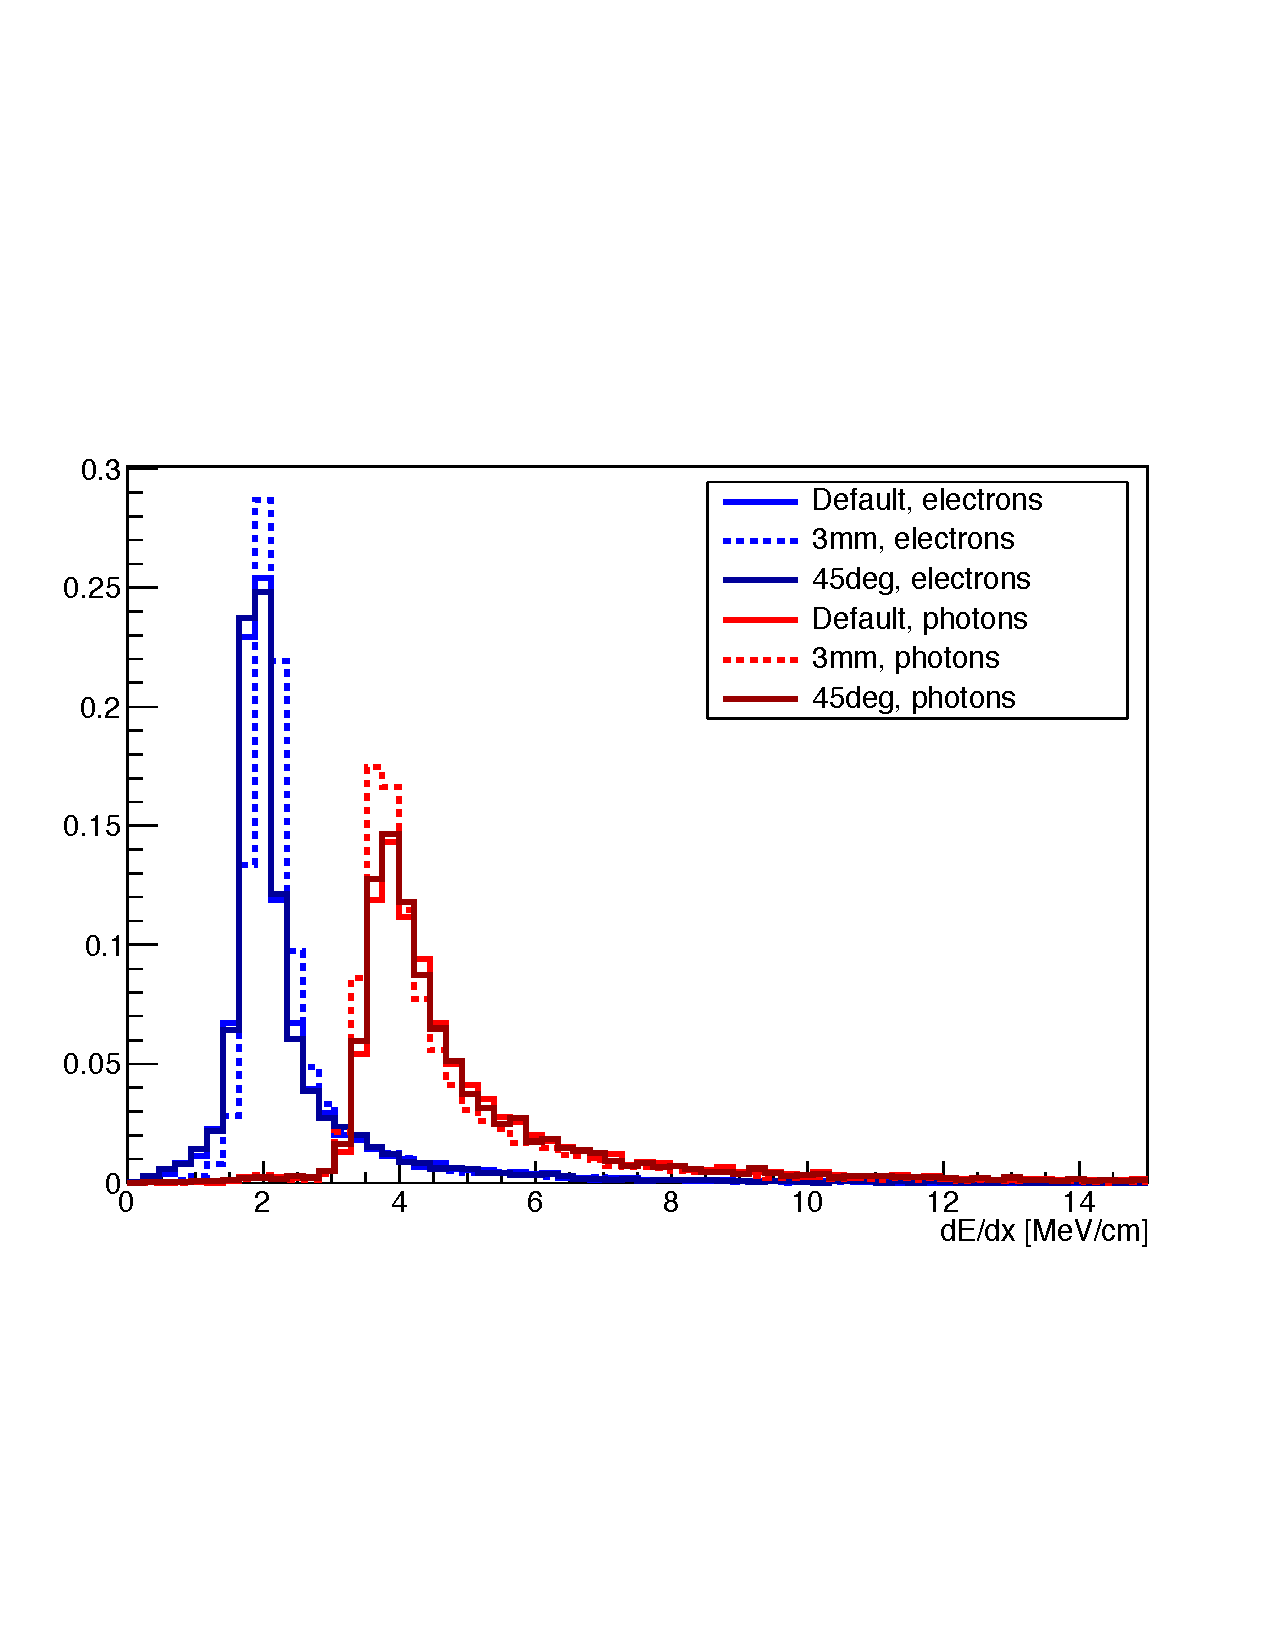
\includegraphics[height=0.24\textheight]{apa-e-gamma-dEdx.pdf} \qquad
(b)
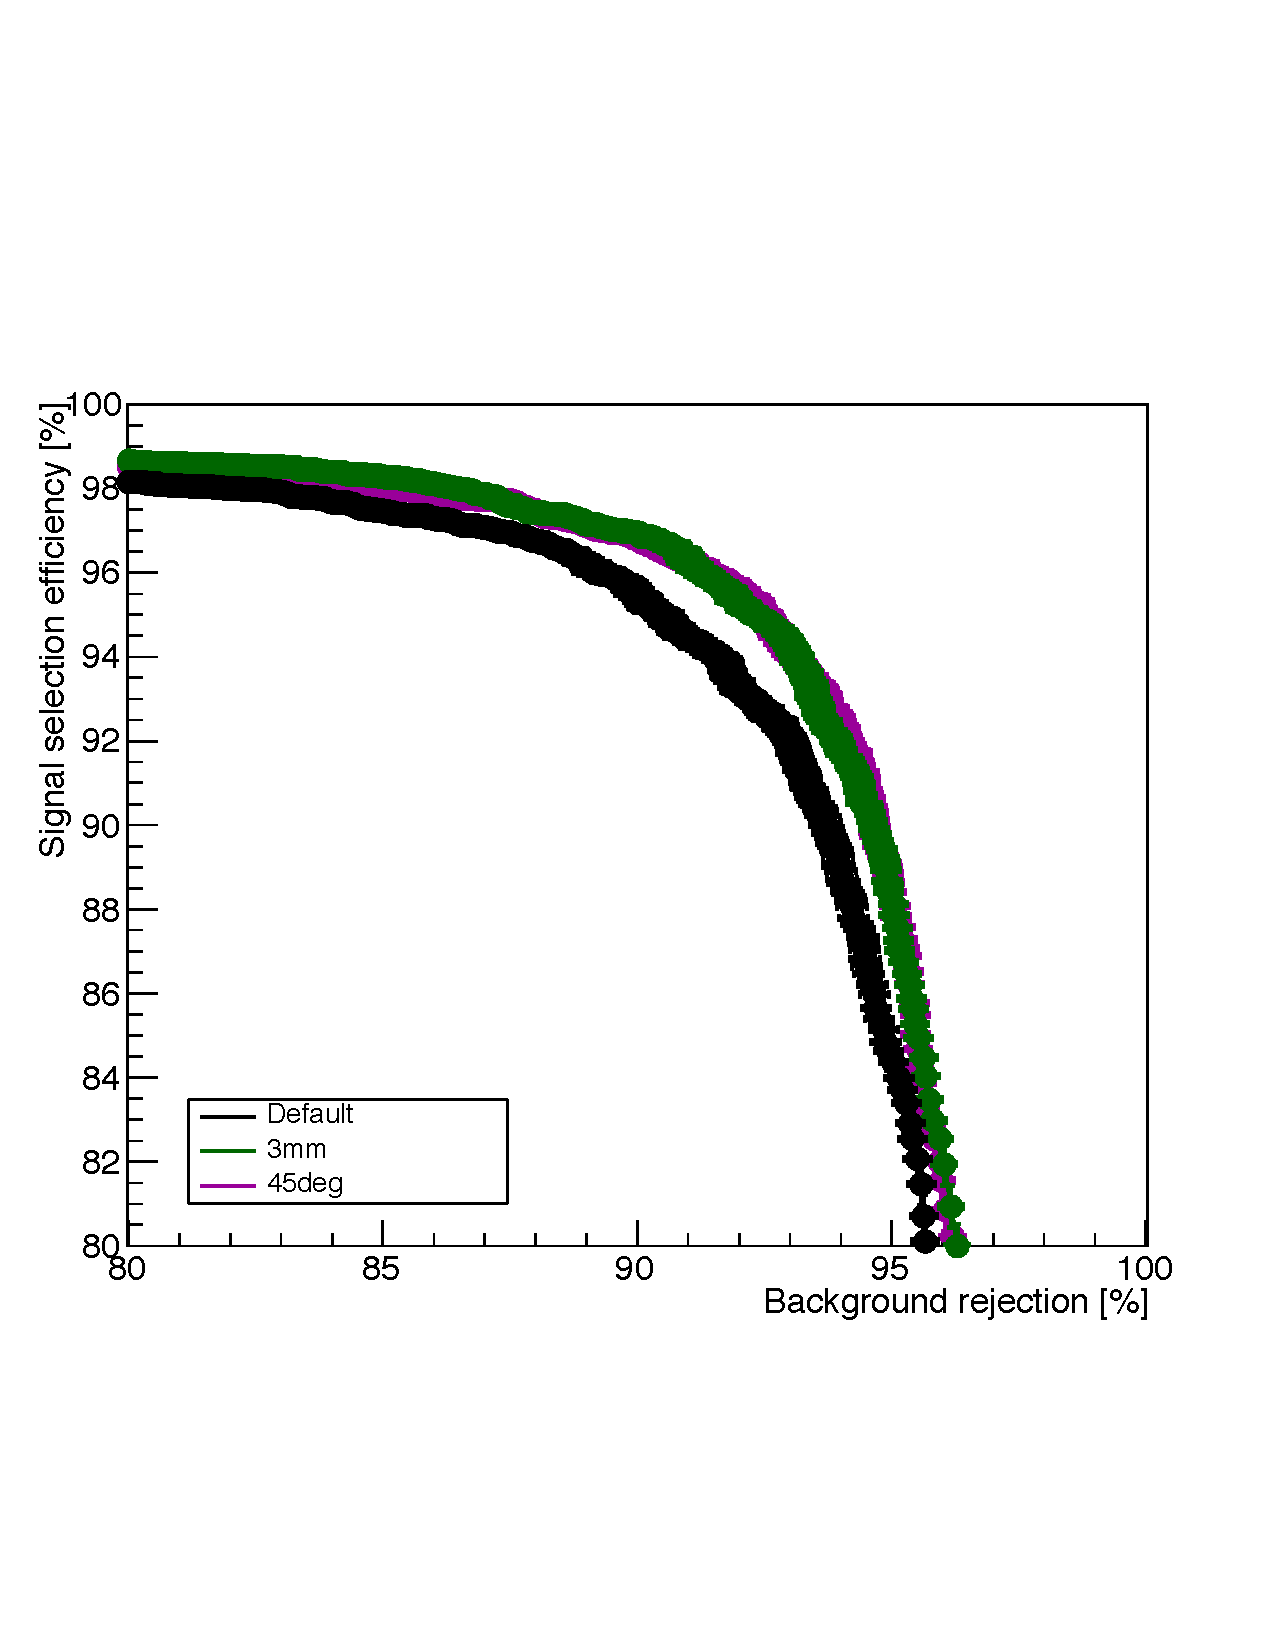
\includegraphics[height=0.24\textheight]{apa-eff-bkgd-wires.pdf} 
\end{dunefigure}

\item \textbf{Wire plane transparency and signal shapes.}  The ordering of the layers, from the outside in, is $G$-$U$-$V$-$X$, followed by the grounding mesh. The operating voltages of the \dword{apa} layers are listed in Table~\ref{tab:bias}.  Figure~\ref{fig:apa-fields} shows the field simulation and expected signal shapes for the bias voltages listed in the table.  When operated at these voltages, the drifting ionization follows trajectories around the grid and induction wires, ultimately terminating on a collection plane wire. The grid and induction layers are completely transparent to drifting ionization, and the collection plane is completely opaque.  The grid layer is present for pulse-shaping purposes and not connected to the electronics readout; it effectively shields the first induction plane from the drifting charge and removes the long leading edge from the signals on that layer. 


\begin{table}[ht]
\begin{minipage}[b]{0.46\linewidth}
\centering
\begin{tabular}{ l  r }
    \hline
    \textbf{Anode Plane} & \textbf{Bias Voltage} \\ \toprowrule
	$G$ - Grid & \SI{-665}{V} \\ \colhline
	$U$ - Induction & \SI{-370}{V{}} \\ \colhline
	$V$ - Induction & \SI{0}{V} \\ \colhline
	$X$ - Collection & \SI{820}{V} \\ \colhline
	Grounding Mesh & \SI{0}{V} \\ \colhline
    \end{tabular}
    \caption{Baseline bias voltages for \dword{apa} wire layers.}
    \label{tab:bias}
\end{minipage}\hfill
\begin{minipage}[t]{0.5\linewidth}
\centering
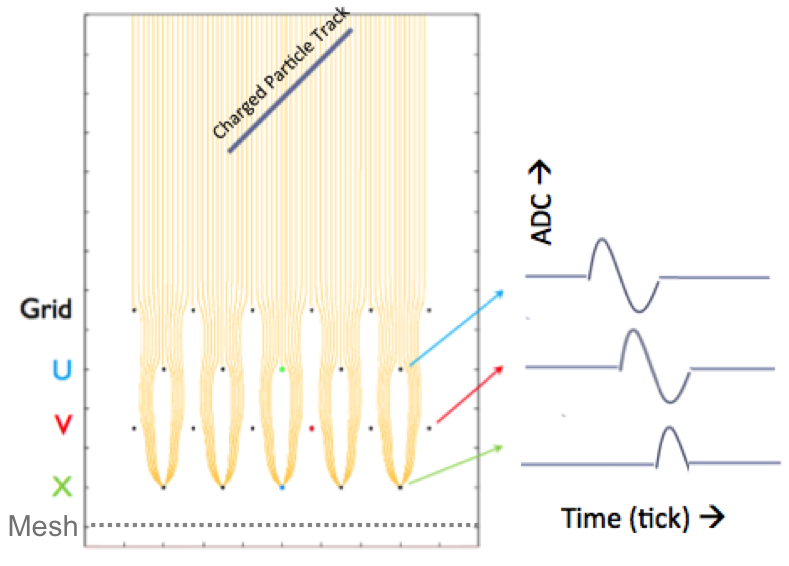
\includegraphics[width=0.9\linewidth]{apa-drawing-wire-field-signals.png}
\captionof{figure}{Field lines and resulting signal shapes on the APA induction and collection wires.}
\label{fig:apa-fields}
\end{minipage}
\end{table}

\item \textbf{Wire type and tension.}  The wire selected for the \dwords{apa} is \SI{150}{$\mu$m} beryllium (\num{1.9}\%) copper wire, %\footnote{\url{http://www.lfa-wire.com/heat-treatable-alloy-25_c17200-and-c17300.htm}}
chosen for its mechanical and electrical properties, ease of soldering, and cost.  The tension on the wires, combined with intermediate support combs (described in Section~\ref{sec:combs}) on the \dword{apa} frame cross beams, ensure that the wires are held taut in place with minimal sag.  Wire sag can impact the precision of reconstruction, as well as the transparency of the TPC wire planes.  The tension must be low enough that when the wires are cooled, which increases their tension due to thermal contraction, they stay safely below the break load of the beryllium copper wire.  To further mitigate wire slippage and its impact on detector performance, each wire in the \dword{apa} is anchored twice at all end points, with both solder and epoxy.  See Section~\ref{sec:fdsp-apa-wires} for more details about the wires.
\end{itemize}

Some of the principal design parameters for the DUNE 
\dwords{apa} are summarized in Table~\ref{tab:apaparameters}.

\begin{dunetable}[\dword{apa} design parameters]{lr}{tab:apaparameters}
{\dword{apa} design parameters}   
Parameter & Value  \\ \toprowrule
Active height & \SI{5.984}{m} \\ \colhline
Active width & \SI{2.300}{m} \\ \colhline
Wire pitch ($U,V$) & \SI{4.669}{mm} \\ \colhline
Wire pitch ($X,G$) & \SI{4.790}{mm} \\ \colhline
Wire pitch tolerance & $\pm$\SI{0.5}{mm} \\ \colhline
Wire plane spacing & \SI{4.75}{mm} \\ \colhline
Wire plane spacing tolerance & $\pm$\SI{0.5}{mm} \\ \colhline
Wire Angle (w.r.t. vertical) ($U,V$) & 35.7$^{\circ}$\\ \colhline
Wire Angle (w.r.t. vertical) ($X,G$) & 0$^{\circ}$\\ \colhline
Number of wires / \dword{apa} & 960 ($X$), 960 ($G$), 800 ($U$), 800 ($V$) \\ \colhline
Number of electronic channels / \dword{apa} & 2560 \\ \colhline
%Wire Tension & \SI{5.0}{N} \\ \colhline
%Wire Tension Tolerance & $\pm$\SI{1}{N} \\ \colhline
Wire material & beryllium copper \\ \colhline
Wire diameter & 150 $\mu$m \\ \colhline
%Wire Resistivity & 7.68 $\mu\Omega$-cm $@$ 20$^{\circ}$ C \\ \colhline
%Wire Resistance/m & 4.4 $\Omega$/m $@$ 20$^{\circ}$ C \\ \colhline
%Frame Planarity & 5 mm \\ \colhline
%Photon Detector Slots & 10 \\
\end{dunetable}


%%%%%%%%%%%%%%%%%%%%%%%%%%%%%%%%%%%%%%%%%%%%%%%%%%%%%%%%%%%%%%%%%%%%%%
\subsection{APA Frames}
\label{sec:fdsp-apa-frames}

The \dword{apa} frames are an assembly of rectangular hollow section (RHS) stainless steel tubes.  As seen in Figure~\ref{fig:apa-frame-2}, there are three long tubes, a foot tube, a head tube, and eight cross-piece ribs that bolt together to create the \SI{6.0}{m} tall by \SI{2.3}{m} wide frame. All hollow sections are \SI{3}{in}. deep with varying widths depending on their role, see Figure~\ref{fig:apa-frame-2}.

\begin{dunefigure}[Bare \dword{apa} frame drawing]{fig:apa-frame-2}
{A \dword{pdsp} \dword{apa} frame showing overall dimensions and the \num{13} separate stainless steel tube sections that bolt together to form a complete frame.  The long tubes and foot tube are 3$\times$\SI{4}{in} cross section, the head tube is 3$\times$\SI{6}{in} and the ribs are \num{3}$\times$\SI{2}{in}. Also shown are the slots and guide rails used to house the light guide bar \dwords{pd} in \dword{pdsp}.}
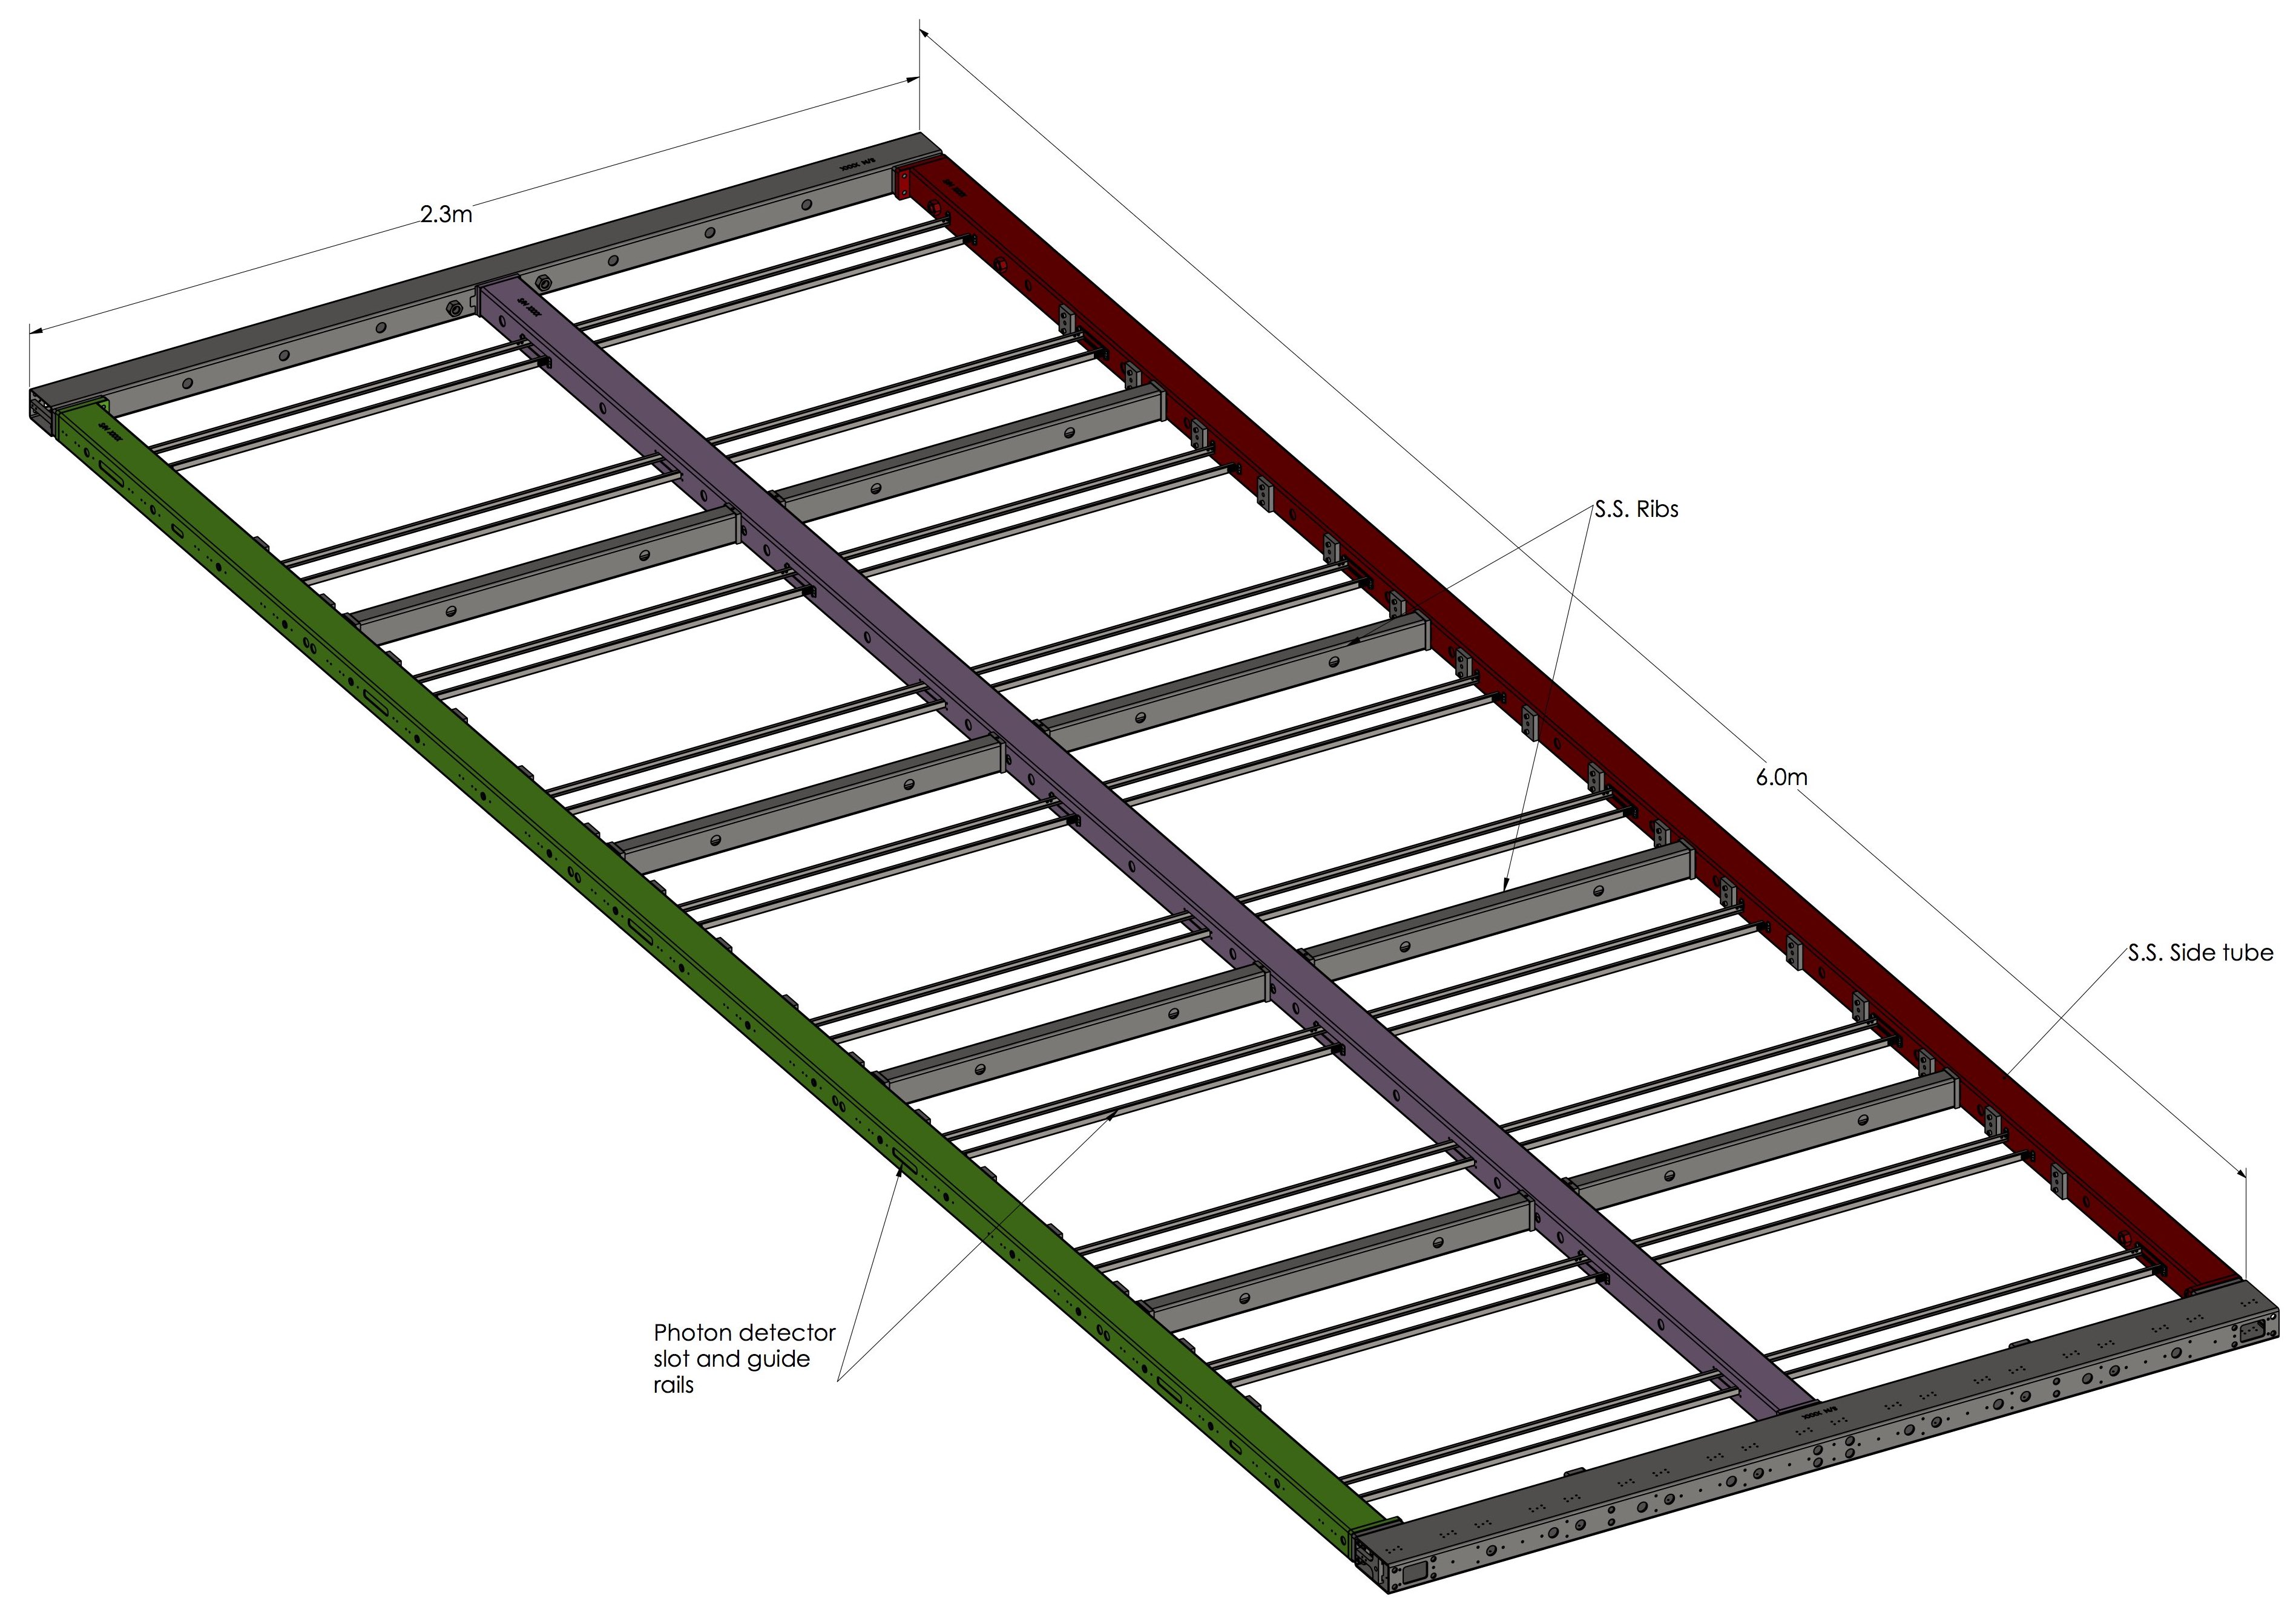
\includegraphics[width=0.9\textwidth]{apa-iso-color.jpg} 
\end{dunefigure}

The head and foot tubes are bolted to the side and center pieces via abutment flanges welded to the tubes. In production, the pieces can be individually machined and cleaned prior to assembly, which gives flexibility both in the production process and helps achieve the flatness and shape tolerances.  During final assembly, shims are used to create a flat, rectangular frame of the specified dimensions.  The central cross pieces are attached to the side pieces in a similar manner.  Figure~\ref{fig:tpc_apa_boltedjointdrawing} shows models of the different joints.   

\begin{dunefigure}[Details of \dword{apa} bolted joints]{fig:tpc_apa_boltedjointdrawing}
{The bolted joints in the \dword{apa} frame. Left: Connection between the head tube and a side tube. Right: Connections between the center tube and the rib pieces on either side.  These bolted connections can be shimmed during assembly to ensure the frame meets dimensional and flatness specifications.}
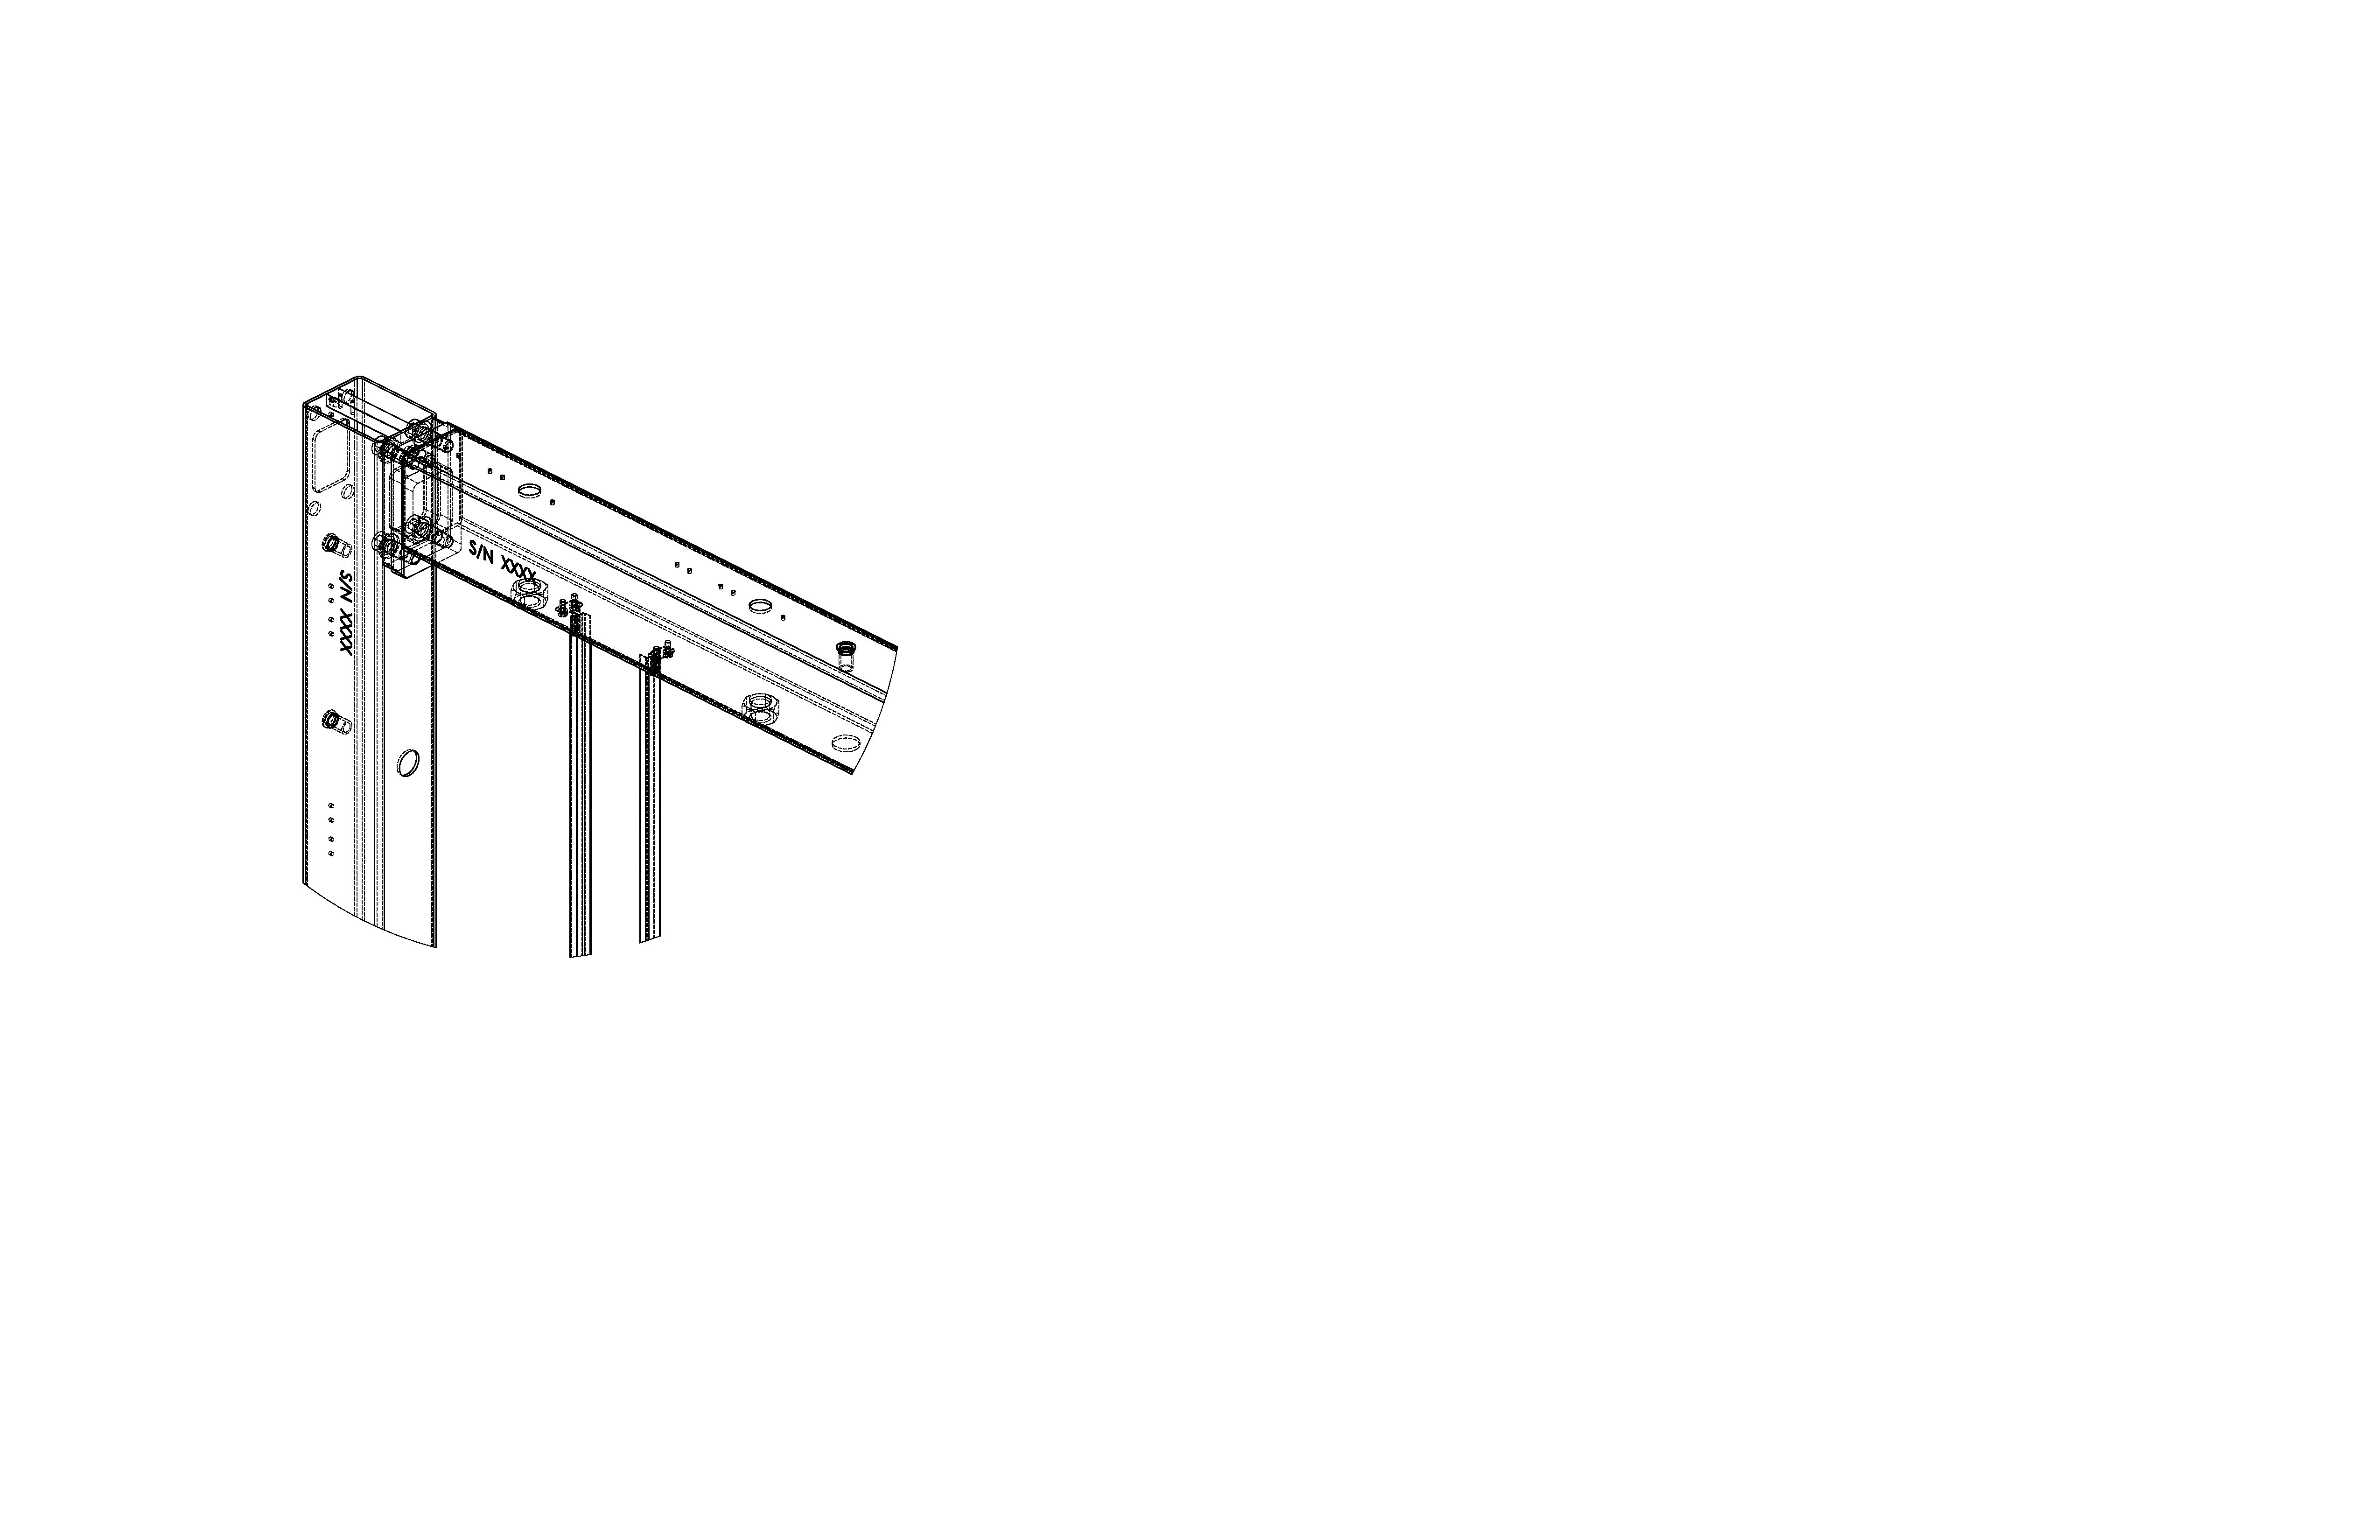
\includegraphics[width=0.45\textwidth]{apa-joint-detail-1.pdf} \quad
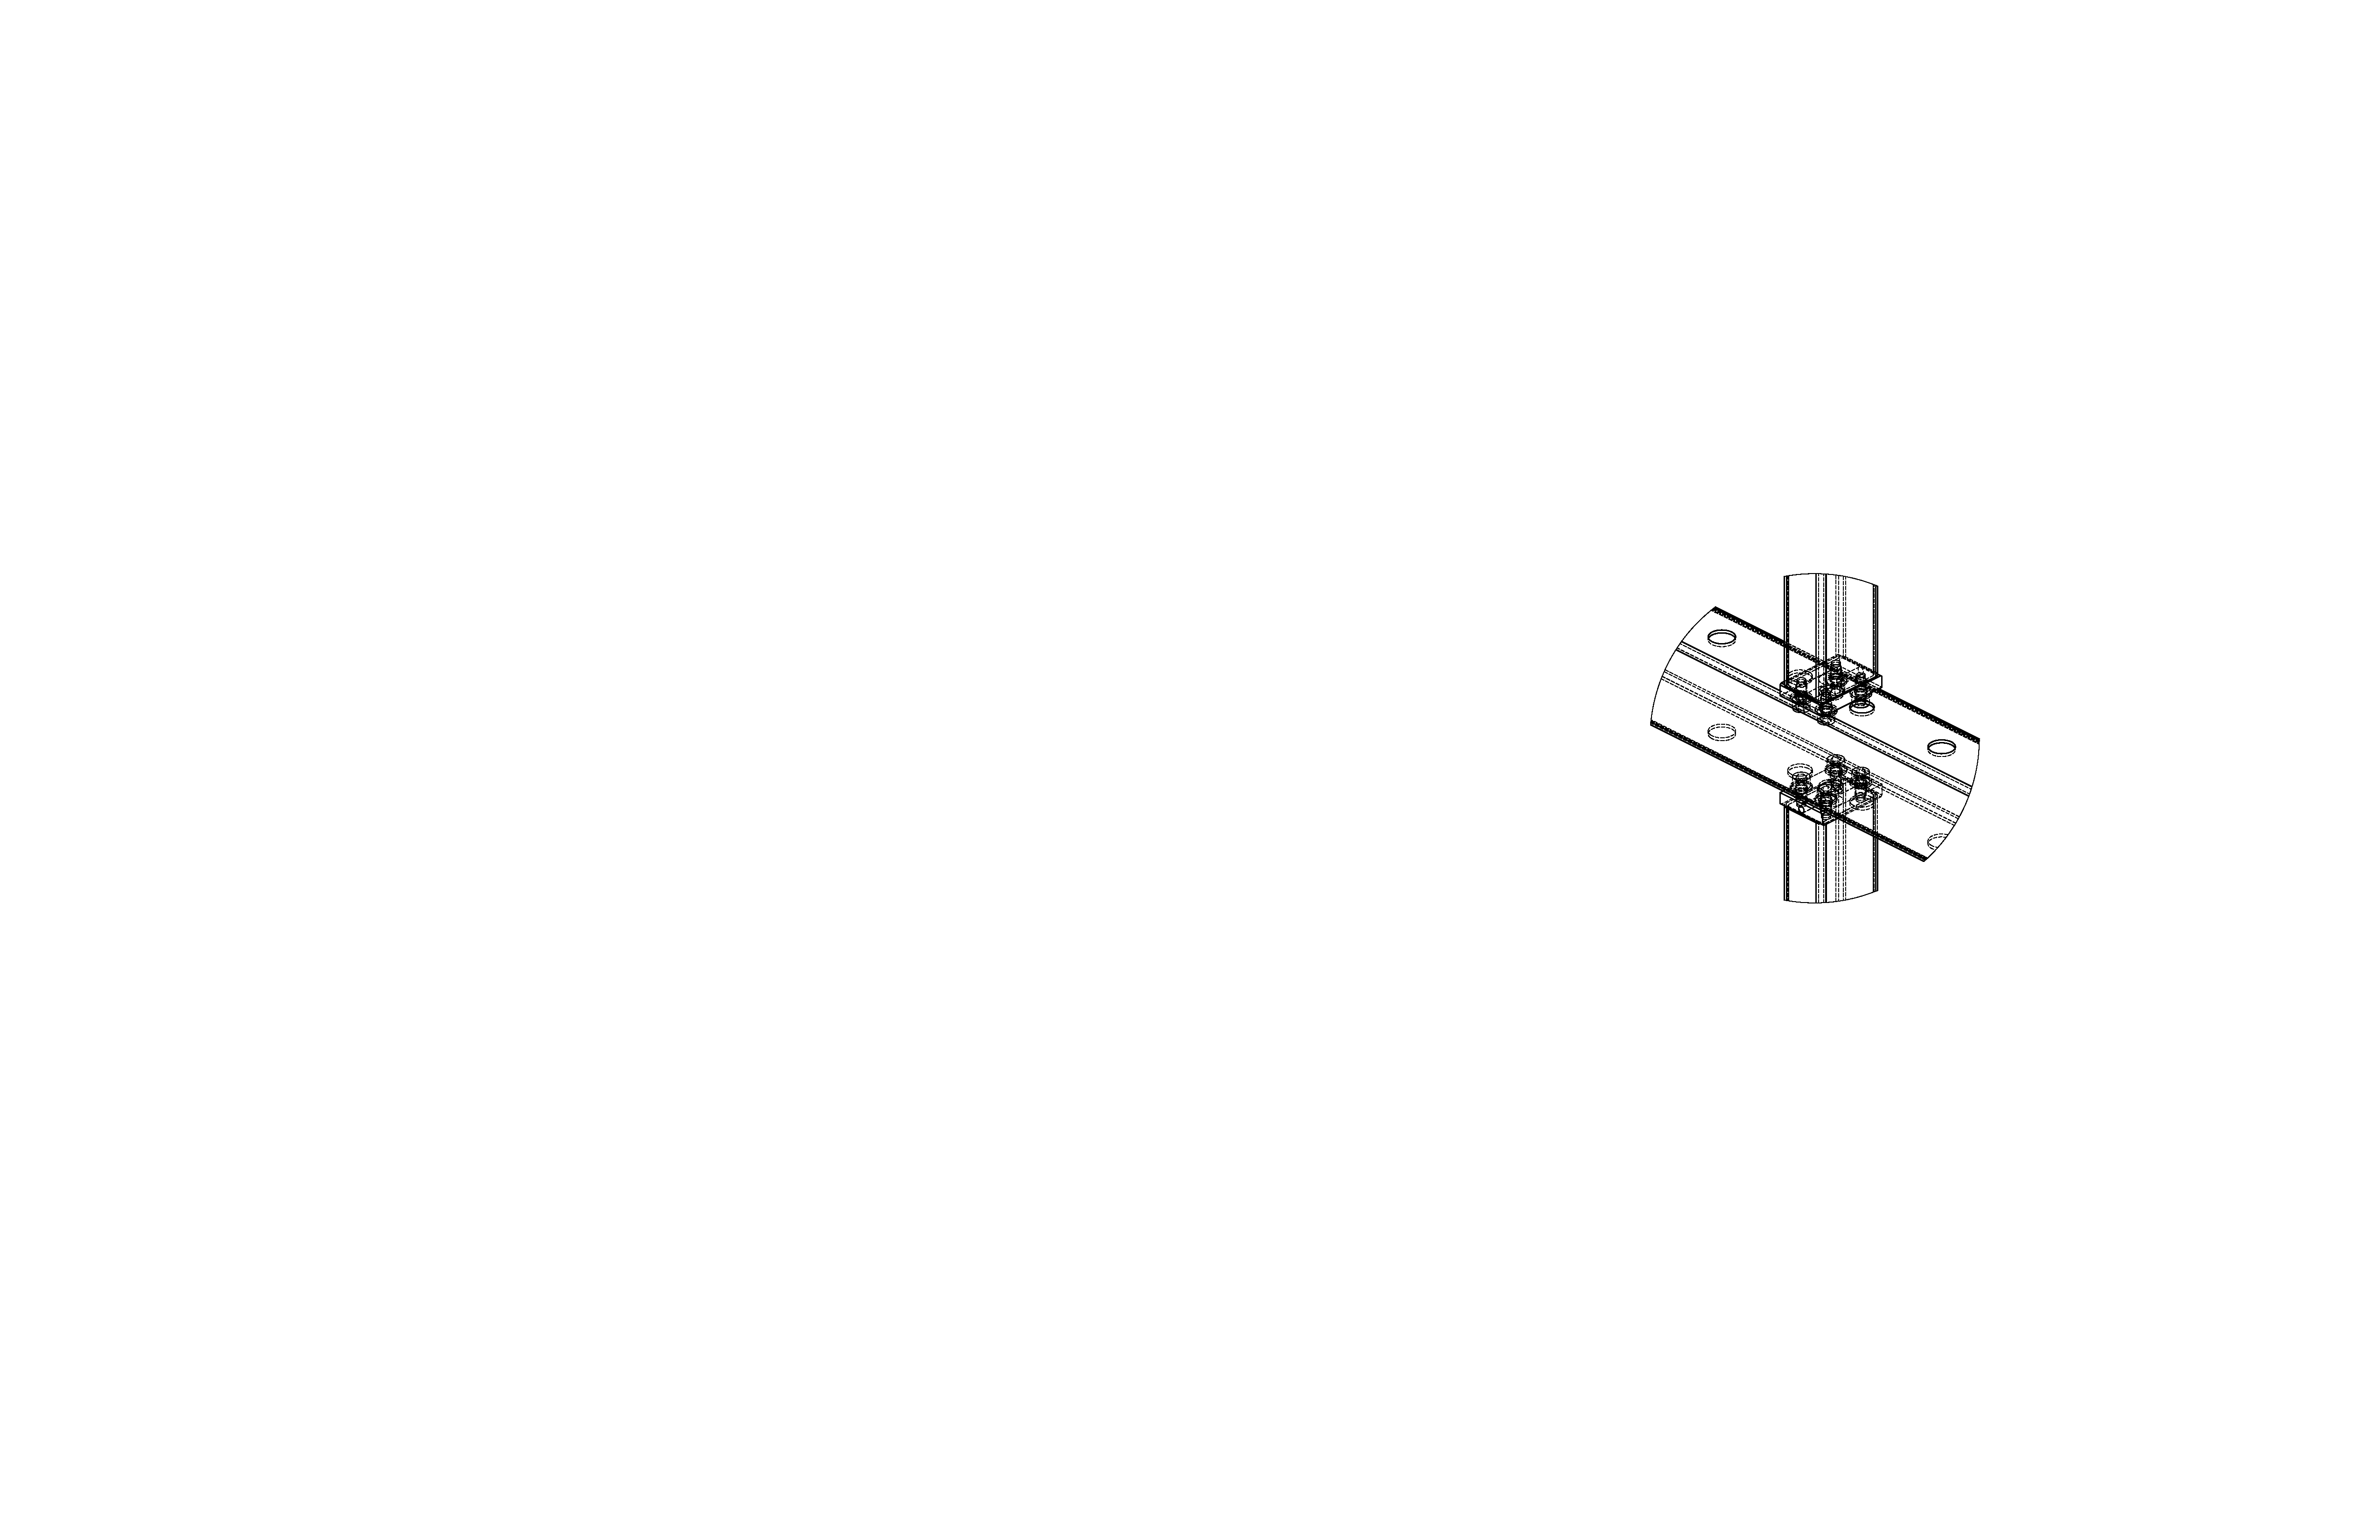
\includegraphics[width=0.45\textwidth]{apa-joint-detail-2.pdf} 
\end{dunefigure}

The \dword{apa} frames also house the \dword{pds}.  In the \dword{pdsp} design, rectangular slots are machined in the outer frame tubes and guide rails are used to secure a light guide bar detector, though alternative \dword{pd} designs are being considered for the \dwords{spmod}. %DUNE. 
(See Section~\ref{sec:fdsp-apa-intfc} for more details on interfacing with the \dword{pds}.)   Also, in a \dword{spmod}, pairs of \dword{apa} frames will be mechanically connected to form a \SI{12}{m} tall structure, as shown in Figure~\ref{fig:tpc_apa_dual}, with electronics for TPC readout located at both the top and bottom of this two-frame assembly and \dwords{pd} installed throughout.  The \dword{apa} frame design, therefore, must support the routing of cables to the top of the detector from both the bottom \dword{apa} readout electronics and the \dwords{pd} mounted throughout both \dwords{apa}.  The dimensions of the stainless steel tube sections used in the frame are currently being revisited from that used in \dword{pdsp} to ensure sufficient space is available to accommodate all detector cables.  See again Section~\ref{sec:fdsp-apa-intfc} on interfaces or Chapter~\ref{fch:fdsp-pd}.
%the Photon Detector Chapter in the \dword{tdr} for more information.

\begin{dunefigure}[Dimensioned diagram of a pair of \dwords{apa} hanging vertically]{fig:tpc_apa_dual}{Diagram of an \dword{apa} pair, with bottom \dword{apa} hung from the top \dword{apa}. The dimensions of the \dword{apa} pair, including the accompanying \dword{ce} (\dword{ce}) and mechanical supports (the yoke), are indicated.}
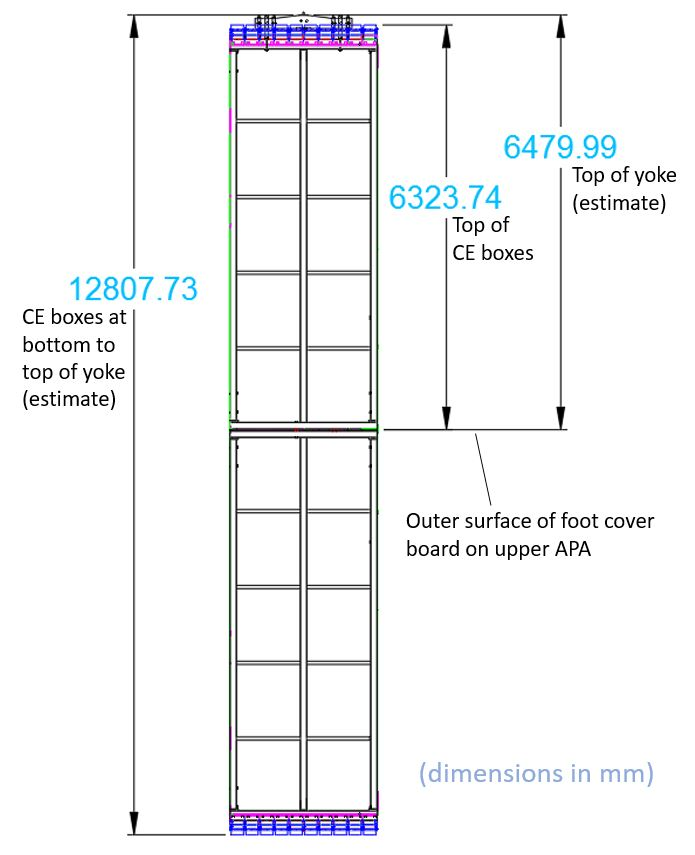
\includegraphics[width=0.9\textwidth]{apa-dual-apas-dimensioned.jpg} 
\end{dunefigure}


%%%%%%%%%%%%%%%%%%%%%%%%%%%%%%%%%%%%%%%%%%%%%%%%%%%%%%%%%%%%%%%%%%%%%
\subsection{Grounding Mesh}
\label{sec:fdsp-apa-mesh}

A fine mesh screen is mounted on both sides of the frames beneath the sense wires to provide a ground plane that evenly terminates the \efield and improves the uniformity of field lines around the wire planes.  This mesh also shields the wires to minimize any potential signal pickup from other detectors.  The mesh used is formed from a %weaved 
woven conducting wire (\SI{80}{$\mu$m} bronze) and is \num{85}\,\% transparent to allow scintillation photons to pass through to the \dwords{pd} mounted inside the frame. 

In the \dword{pdsp} \dwords{apa}, the mesh was installed in four parts, along the length of the left- and right-hand halves of each side of the \dword{apa}. The mesh was clamped around the perimeter of the opening and then pulled tight (by opening and closing clamps, as needed, during the process).  Once the mesh was taut, a \SI{25}{mm} wide strip was masked off around the opening and epoxy was applied through the mesh to attach it directly to the steel frame.  Although measurements have shown that this gives good electrical contact between the mesh and the frame, a deliberate electrical connection was also made.  Figure~\ref{fig:tpc-apa-mesh-application} depicts the mesh application setup for a full-size \dword{pdsp} \dword{apa}.

\begin{dunefigure}[Photos of \dword{apa} grounding mesh application in \dword{pdsp}]{fig:tpc-apa-mesh-application}
{Grounding mesh being clamped to the \dword{apa} and taped off, ready for gluing to a ProtoDUNE-SP frame.}
\setlength{\fboxsep}{0pt}
\setlength{\fboxrule}{0.5pt}
\fbox{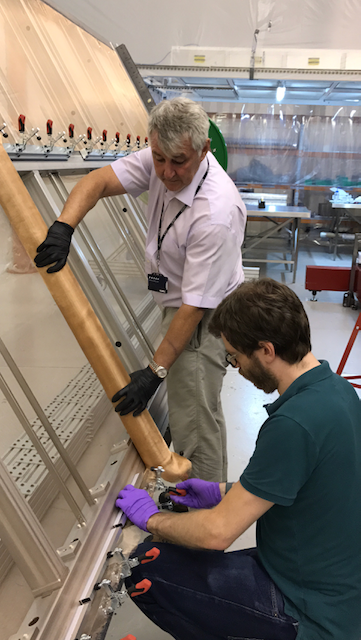
\includegraphics[height=0.6\textwidth]{apa-mesh-application.png}
} \quad
\fbox{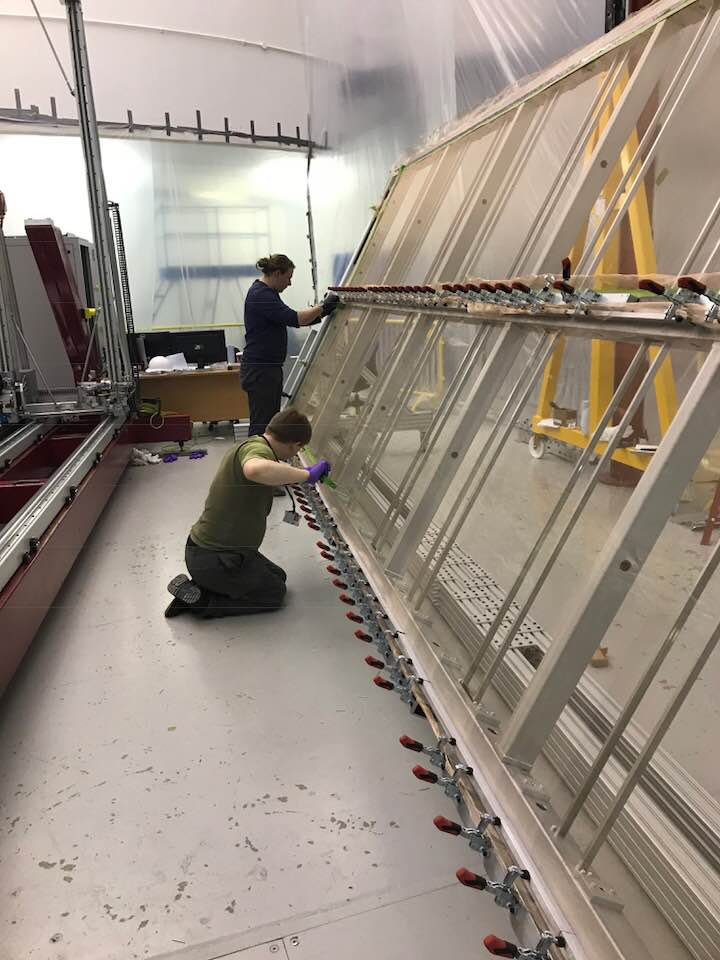
\includegraphics[height=0.6\textwidth]{apa-mesh-applied.jpg}
}
\end{dunefigure}
\fixme{Replacing ProtoDUNE-SP in the caption with the dword generated an error. Don't know why. Anne}

The mesh installation procedure described above is difficult and prone to wrinkles remaining %being left 
in the mesh that can affect the \efield uniformity and the transparency of the wire planes. For the DUNE mass production, a window-frame design is being considered, where mesh is pre-stretched over smaller sub-frames that can be clipped into each gap between cross beams in the full \dword{apa} frame.  See Section~\ref{sec:fdsp-apa-prod-assy} for more information.


%%%%%%%%%%%%%%%%%%%%%%%%%%%%%%%%%%%%%%%%%%%%%%%%%%%%%%%%
\subsection{Wires}
\label{sec:fdsp-apa-wires}

The \SI{150}{$\mu$m} (\SI{.006}{in}) diameter beryllium copper (CuBe) wire chosen for use in the \dwords{apa} is known for its high durability and yield strength. It is composed of \num{98}\,\% copper, \num{1.9}\,\% beryllium, and a negligible amount of other elements. Each \dword{apa} contains a total of \SI{23.4}{km} of wire.  

The key properties for its use in the \dwords{apa} are low resistivity, high tensile or yield strength, and a coefficient of thermal expansion suitable for use with the \dword{apa}'s stainless steel frame (see Table~\ref{tab:wire} for a summary of properties).  Tensile strength of the wire describes the wire-breaking stress.  The yield strength is the stress at which the wire starts to take a permanent (inelastic) deformation, and is the important limit stress for this case.  The wire purchased from Little Falls Alloys~\footnote{Little Falls Alloys\texttrademark, \url{http://www.lfa-wire.com/}} for use on \dword{pdsp} had tensile strength over \SI{1380}{MPa} and yield strength more than \SI{1100}{MPa} (\SI{19.4}{N} for \SI{150}{$\mu$m} diameter wire).  The stress while in use is around \SI{280}{MPa} (\SI{5}{N}), leaving a comfortable margin.

The coefficient of thermal expansion (CTE) describes how a material expands or contracts with changes in temperature.  The CTEs of CuBe alloy and \num{304} stainless steel are very similar.  Integrated down to \SI{87}{K}, they are \SI{2.7}{mm/m} for stainless steel and \SI{2.9}{mm/m} for CuBe. Since the wire contracts slightly more than the frame, for a wire starting at \SI{5}{N} at room temperature, for example, the tension increases to around \SI{5.5}{N} when everything reaches \lar temperature.  

The change in wire tension during cool-down is also important to consider.  In the worst case, the wire cools quickly to \SI{87}{K} before any significant cooling of the much larger frame.  In the limiting case with complete contraction of the wire and none in the frame, the tension would peak around \SI{11.7}{N}, which is still well under the \SI{20}{N} yield tension. In practice, however, the cooling will be done gradually to avoid this tension spike as well as other thermal shocks to the detectors.

\begin{dunetable}[Beryllium copper (CuBe) wire properties]{lr}{tab:wire}{Summary of properties of the beryllium copper wire used on the \dwords{apa}.}
Parameter & Value \\ \toprowrule
Resistivity & 7.68 $\mu\Omega$-cm $@$ 20$^{\circ}$ C \\ \colhline
Resistance & 4.4 $\Omega$/m $@$ 20$^{\circ}$ C \\ \colhline
Tensile strength (from property sheets)  & \SI{1436}{MPa} / \SI{25.8}{N} for \SI{150}{$\mu$m} wire \\ \colhline
%Tensile strength (from actual wire)  & \SI{212530}{psi} / \SI{26.4}{N} for \SI{150}{$\mu$m} wire \\ \colhline
CTE of beryllium copper integrated to \SI{87}{K}  & \SI{2.9e-3}{m/m} \\ \colhline
CTE of stainless steel integrated to \SI{87}{K}  & \SI{2.7e-3}{m/m} \\
\end{dunetable}



%%%%%%%%%%%%%%%%%%%%%%%%%%%%%%%%%%%%%%%%%%%%%%%%%%%%%%%%%%%%%%%%
\subsection{Wire Boards and Anchoring Elements}
\label{sec:fdsp-apa-boards}

To guide and secure the \num{3520} wires on an \dword{apa}, stacks of custom FR4 circuit boards attach to the outside edges of the frame, as shown in the engineering drawings in Figure~\ref{fig:apa-wire-boards}.  There are \num{204} \textit{wire boards} on each \dword{apa} and \num{337} total circuit boards, where this number includes the wire boards, cover boards, capacitive-resistive (CR) boards, $G$-layer bias boards, adapter boards, and one SHV board.

\begin{dunefigure}[Wire carrier board layout on the \dword{apa} frames]{fig:apa-wire-boards}
{Engineering drawings that illustrate the layering of the wire carrier boards that are secured along the perimeter of the \dword{apa} steel frames. Left: The full set of $V$-layer boards.  Right: Detail showing the full stack of four boards at the head end of the \dword{apa}.}
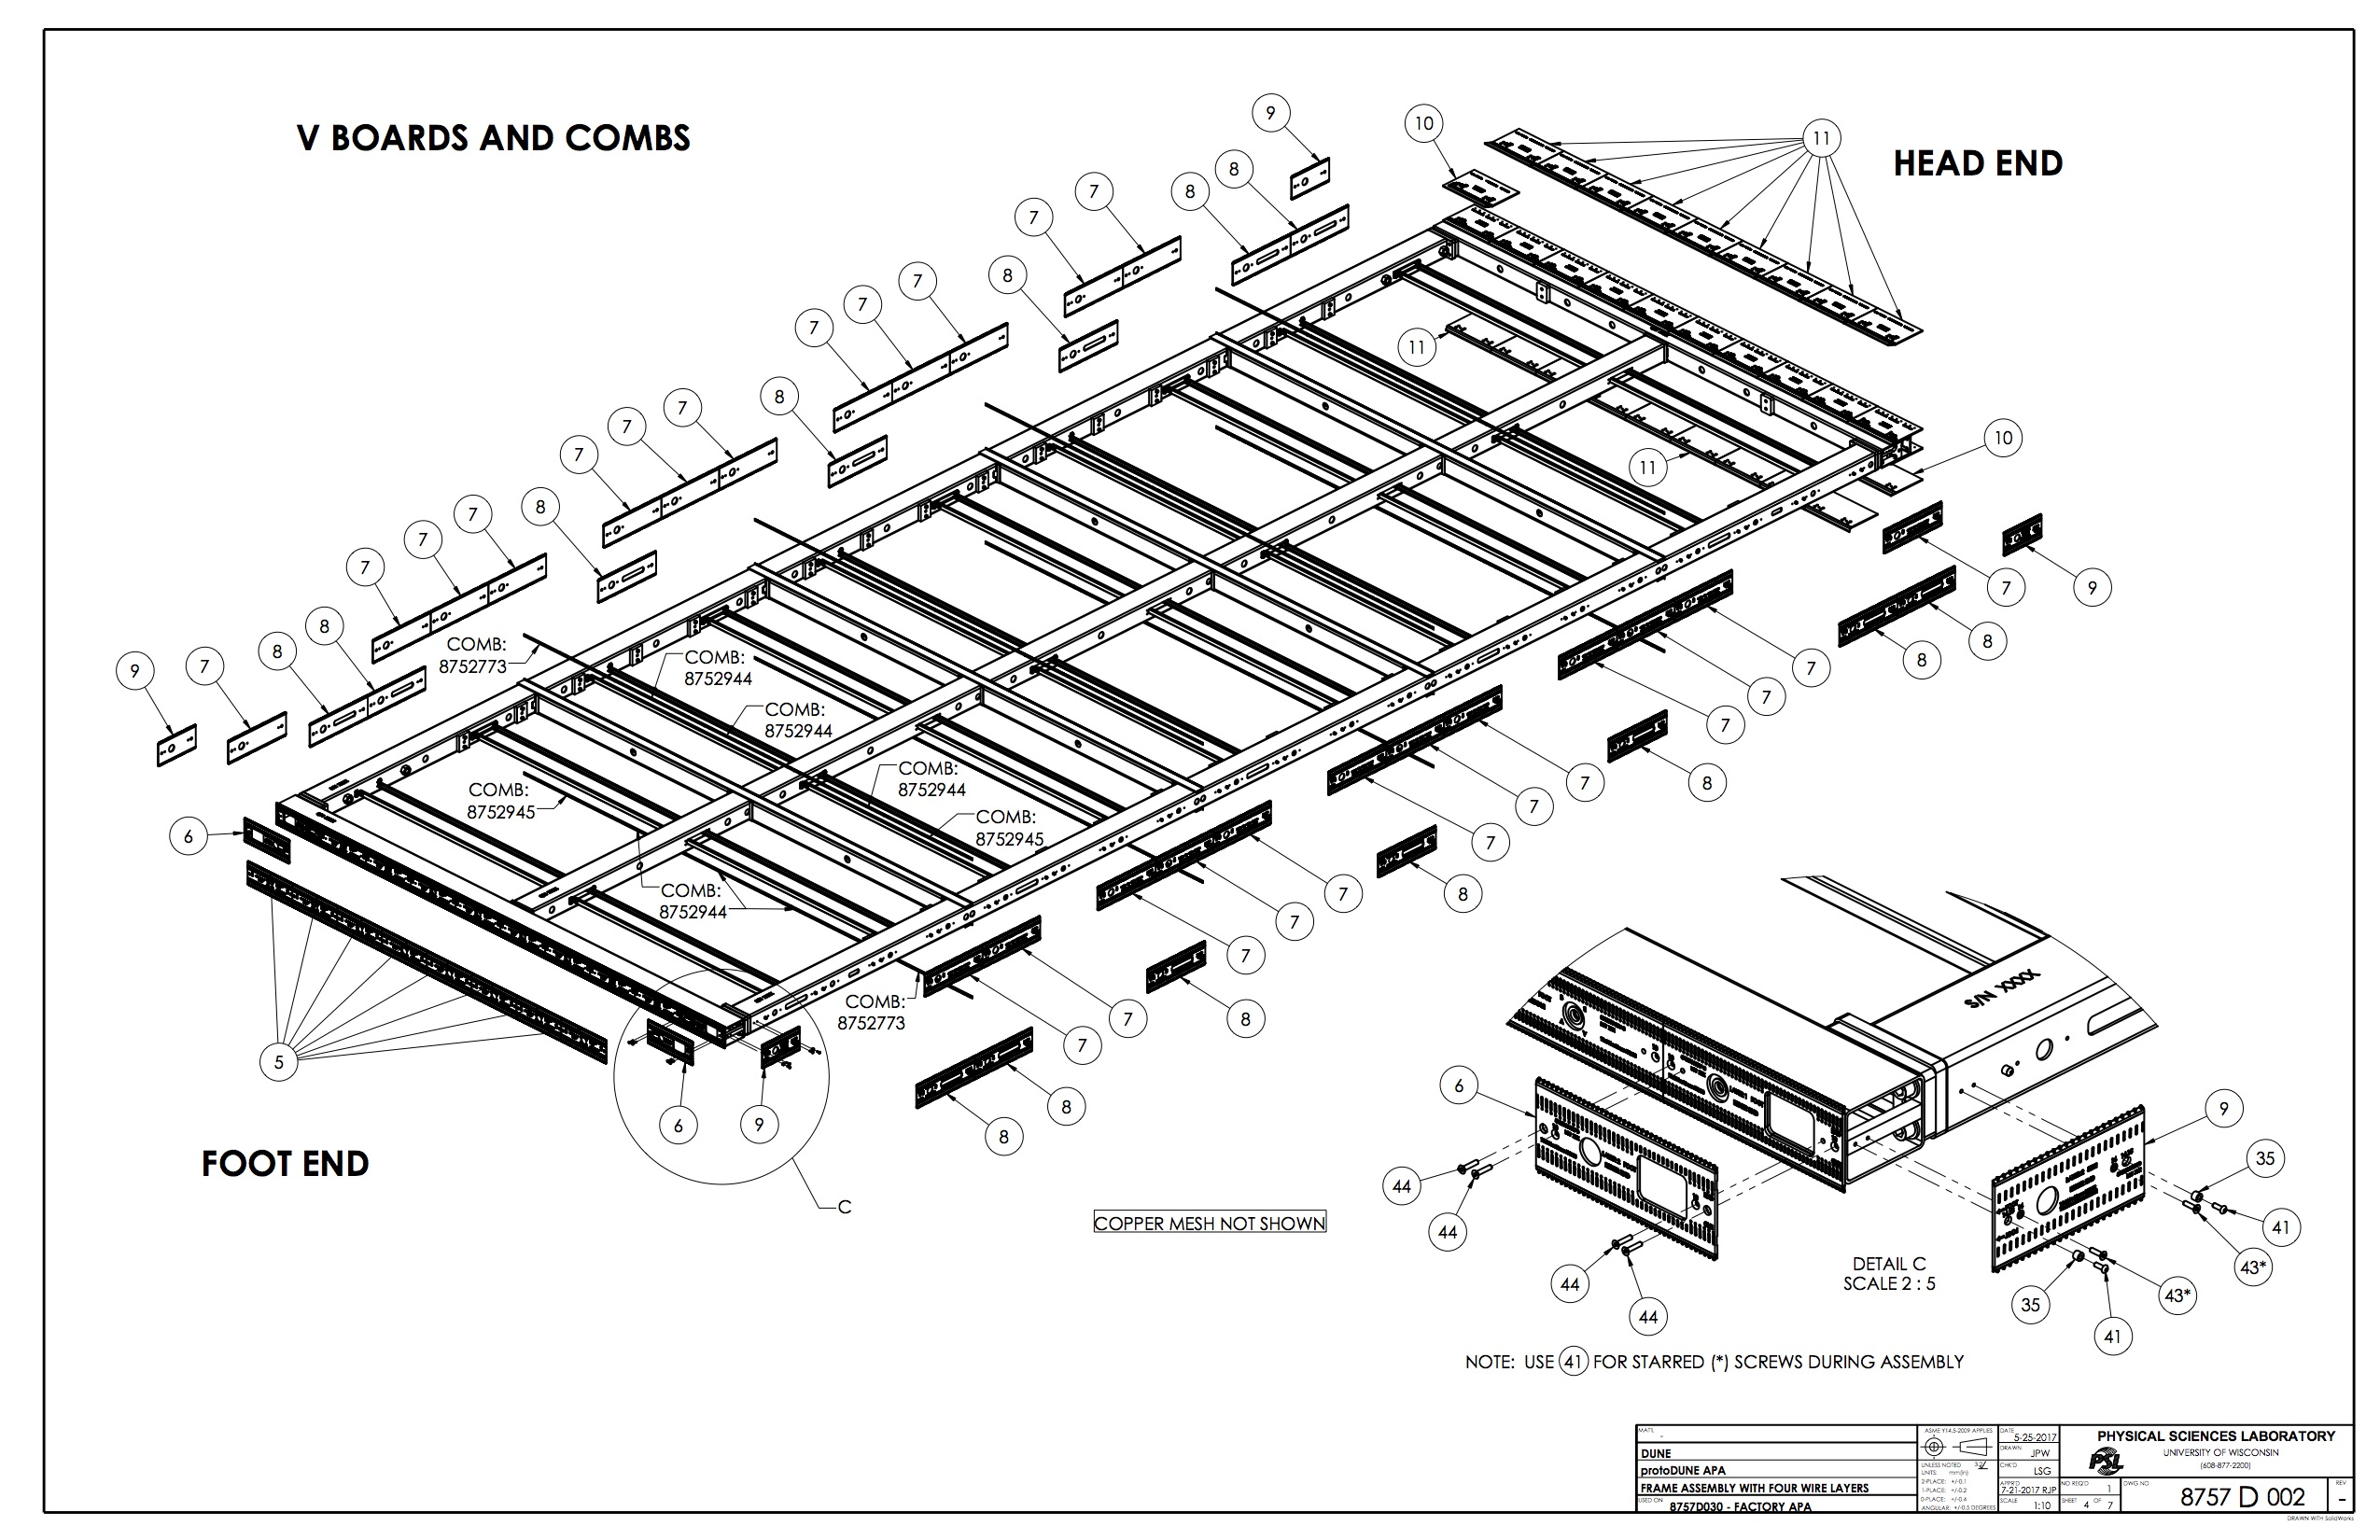
\includegraphics[width=0.48\textwidth]{apa-drawing-v-boards-exploded.jpg}
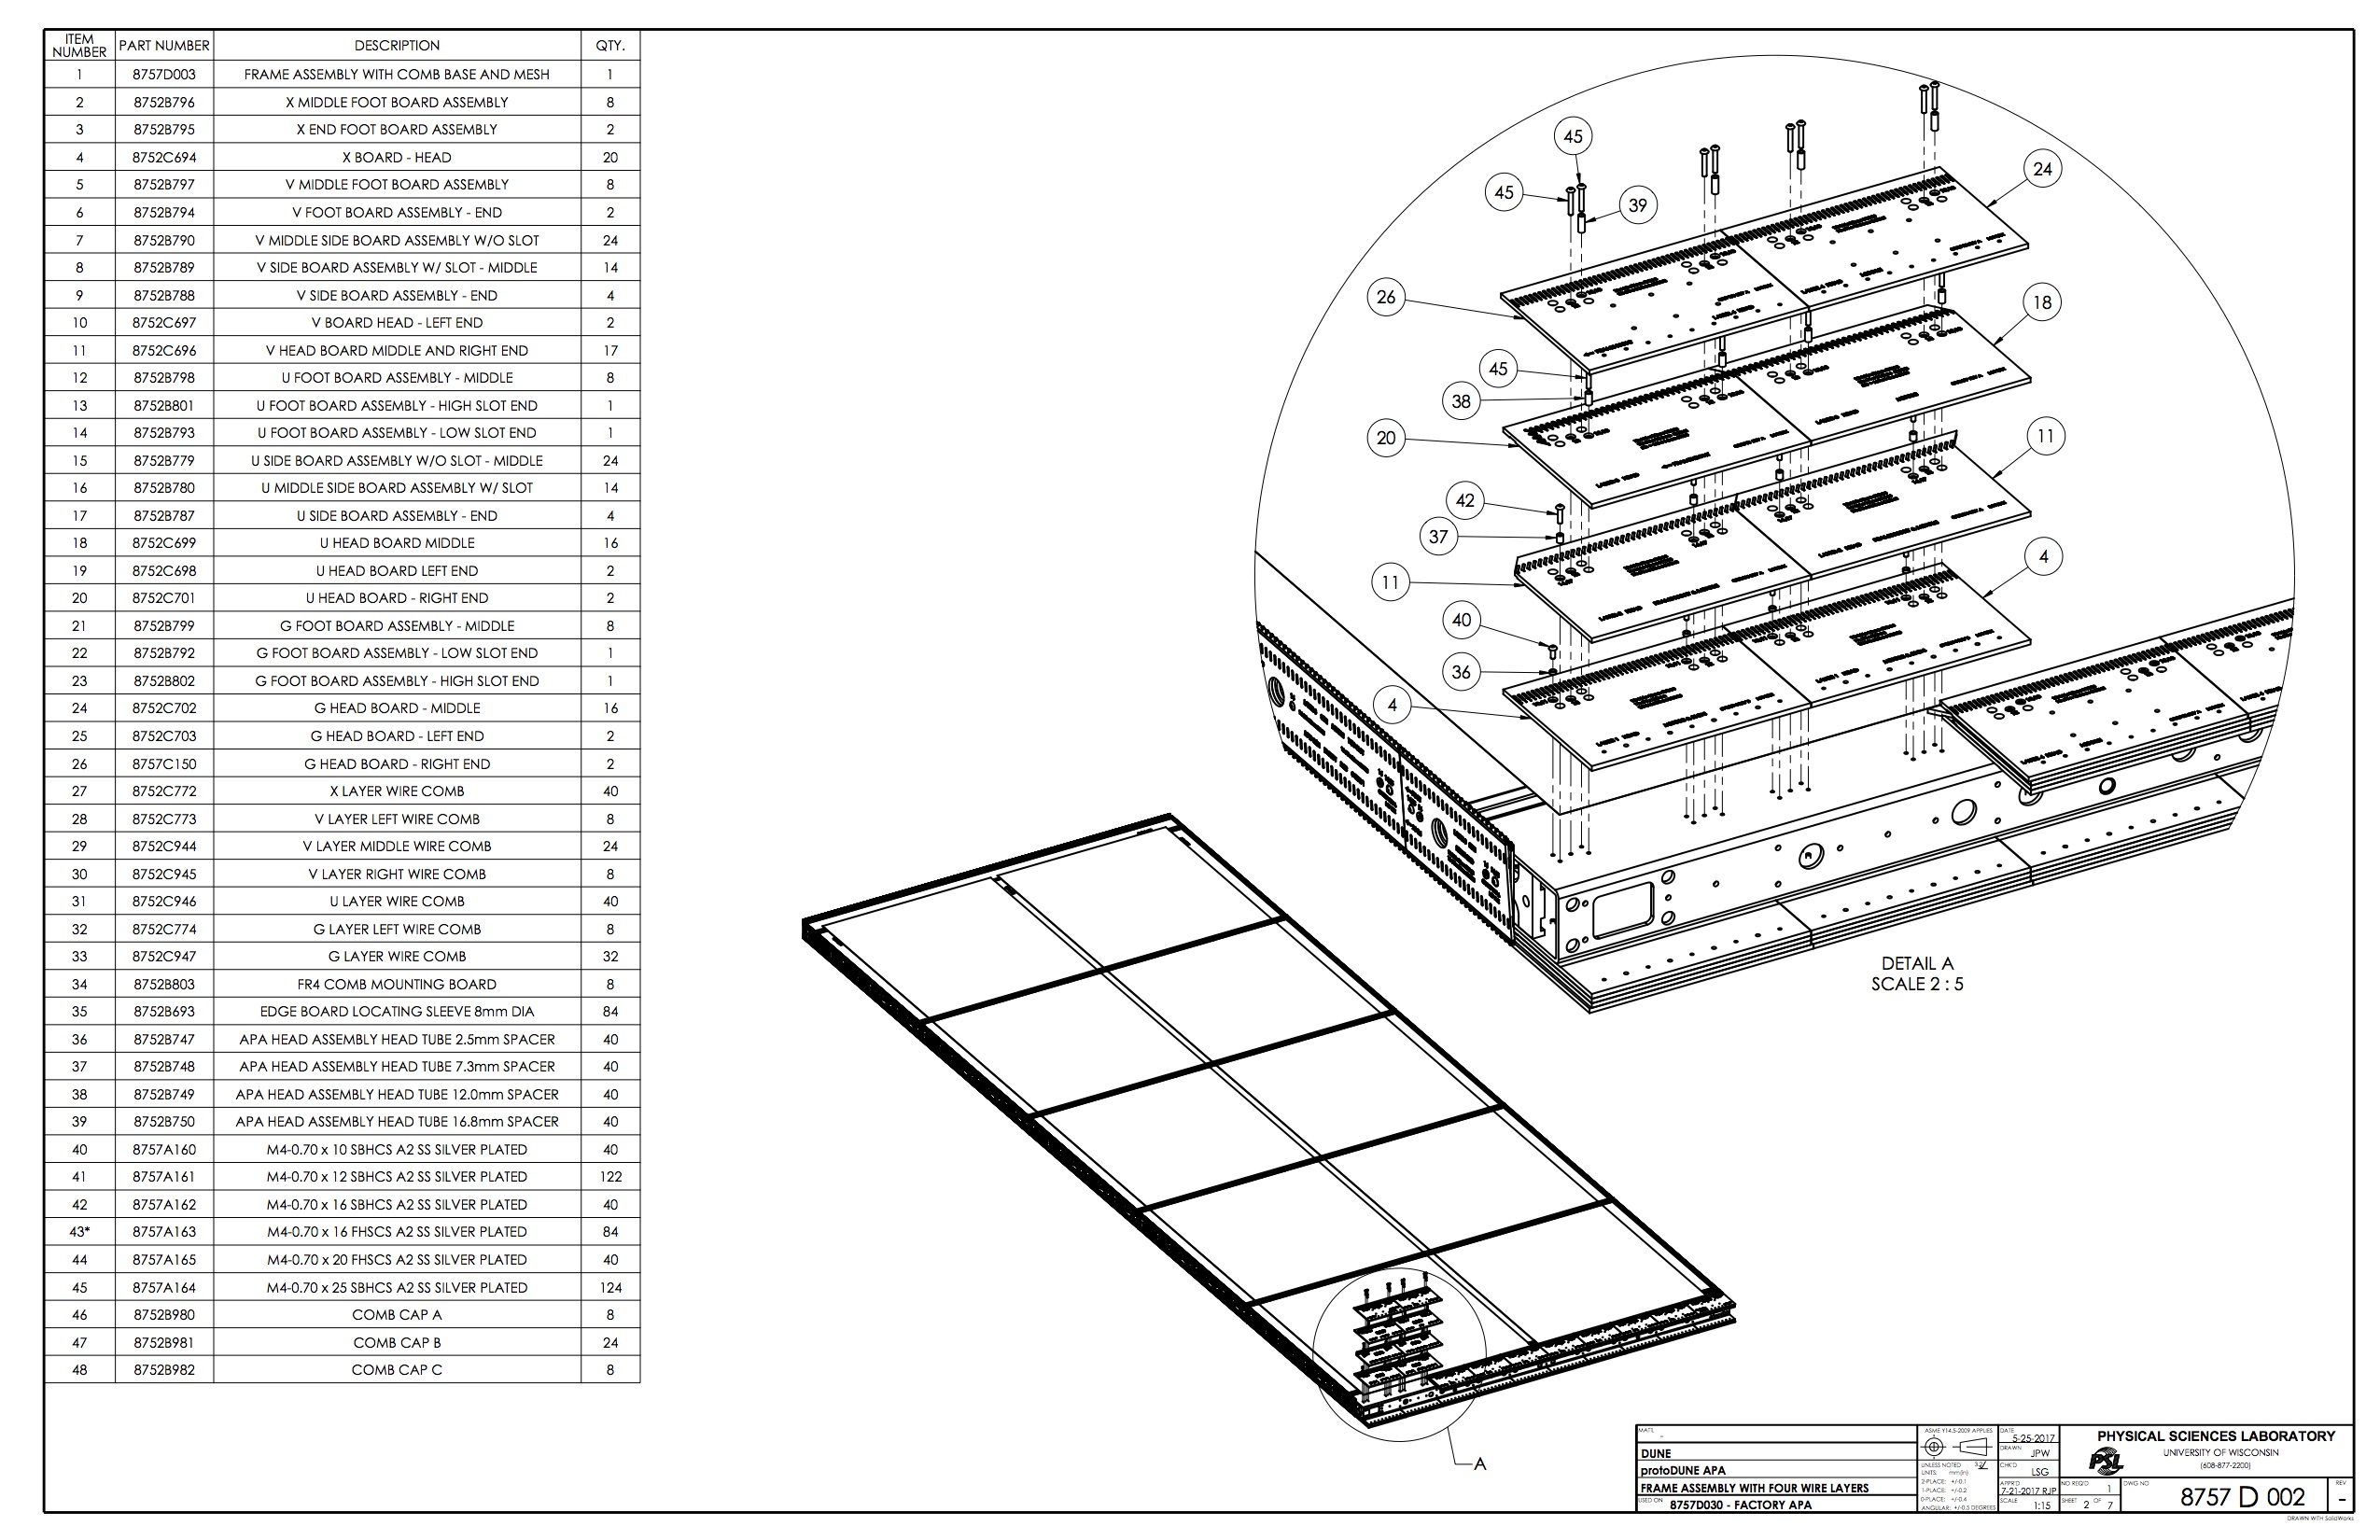
\includegraphics[width=0.48\textwidth]{apa-drawing-board-stack-detail.jpg}
\end{dunefigure}


%%%%%%%%%%%%%%%%%%%%%%%%%%%%%%%%%%%%%%%
\subsubsection{Head Electronics Boards}

All \dword{apa} wires are terminated on wire boards that are stacked along the electronics end of the \dword{apa} frame.  The board stack at the head end is shown in Figure~\ref{fig:apa-wire-boards}. Attachment of the wire boards begins with the $X$-plane (lowest). Once the $X$-plane wires are strung on both sides of the \dword{apa} frame, they are soldered and epoxied to their wire boards and trimmed. The remaining wire board layers are attached as each previous layer of wires are placed.  The wire plane spacing of \SI{4.75}{mm} is set by the thickness of these wire boards.   

Mill-Max~\footnote{Mill-Max\texttrademark{}, \url{https://www.mill-max.com/}} pins and sockets provide electrical connections between circuit boards within a stack. They are pressed into the circuit boards and are not repairable if damaged. To minimize the possibility of damaged pins, the boards are designed so that the first wire board attached to the frame has only sockets. All boards attached subsequently contain pins that plug into previously mounted boards. This process eliminates exposure of any pins to possible damage during winding, soldering, or trimming processes.

The $X$, $U$ and $V$ layers of wires are connected to the \dword{ce} (housed in boxes mounted on the \dword{apa}) either directly or through DC-blocking capacitors.  Ten stacks of wire boards are installed across the width of each side along the head of the \dword{apa}.  The $X$-layer board in each stack has room for \num{48} wires, the $V$-layer has 40 wires, the $U$-layer \num{40} wires and the $G$-layer \num{48} wires.  Each board stack, therefore, has 176 wires but only \num{128} signal channels since the $G$ wires are not read out. With a total of \num{20} stacks per \dword{apa}, this results in \SI{2560} signal channels per \dword{apa} and a total of \SI{3520} wires starting at the top of the \dword{apa} and ending at the bottom. Many of the capacitors and resistors that in principle could be on these wire boards are instead placed on the attached CR boards (see next section) to improve their accessibility in case of component failure. Figure~\ref{fig:tpc_apa_electronics_connectiondiagram} depicts the connections between the different elements of the \dword{apa} electrical circuit at the head end of the frame. 

\begin{dunefigure}[\dword{apa} wire board connection to electronics]{fig:tpc_apa_electronics_connectiondiagram}{The wire board stack at the head end of an \dword{apa} and the connection to the \dword{ce}. The set of wire boards within a stack can be seen on both sides of the \dword{apa}, with the CR board extending further to the right to provide a connection to the \dword{ce}.}
\setlength{\fboxsep}{0pt}
\setlength{\fboxrule}{0.5pt}
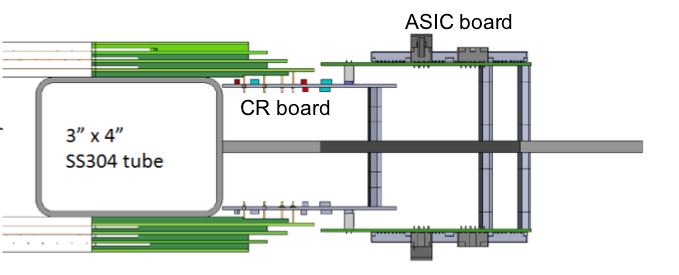
\includegraphics[width=0.62\textwidth, trim=0mm 0mm 5mm 0mm, clip]{apa-board-connections.png}
\fbox{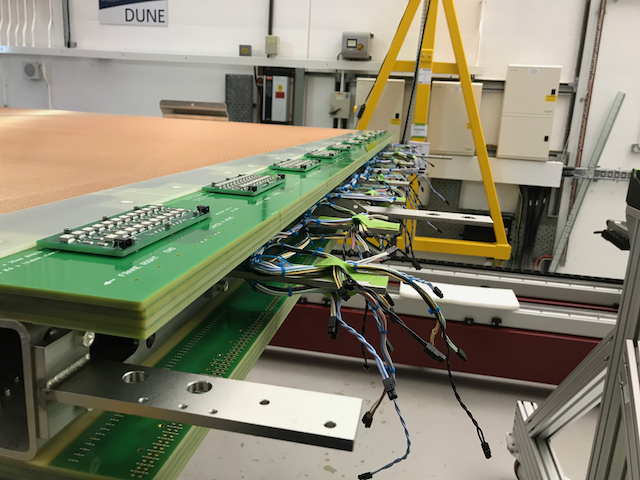
\includegraphics[width=0.37\textwidth]{apa-board-stack.png}
}
\end{dunefigure} 


%%%%%%%%%%%%%%%%%%%%%%%%%%
\subsubsection{CR Boards}
\label{sec:crboards}

The capacitive-resistive (CR) boards carry a bias resistor and a DC-blocking capacitor for each wire in the $X$ and $U$-planes. These boards are attached to the board stacks after fabrication of all wire planes.   Electrical connections to the board stack are made though Mill-Max pins that plug into the wire boards. Connections from the CR boards to the \dword{ce} are made through a pair of \num{96}-pin Samtec~\footnote{Samtec\texttrademark \url{https://www.samtec.com/}} connectors.

Surface-mount bias resistors on the CR boards have resistance of \SI{50}{\mega\ohm} and are constructed with a thick film on a ceramic substrate. Rated for \SI{2.0}{kV} operation, the resistors measure \num{3.0}$\times$\SI{6.1}{mm} (\num{0.12}$\times$\SI{0.24}{in}). The selected DC-blocking capacitors have capacitance of \SI{3.9}{nF} and are rated for \SI{2.0}{kV} operation. Measuring \num{5.6}$\times$\SI{6.4}{mm} (\num{0.22}$\times$\SI{0.25}{in}) across and \SI{2.5}{mm} (\SI{0.10}{in}) high, the capacitors feature flexible terminals to comply with PC board expansion and contraction. They are designed to withstand \num{1000} thermal cycles between the extremes of the operating temperature range. Tolerance is also \num{5}\,\%.

In addition to the bias and DC-blocking capacitors for all $X$ and $U$-plane wires, the CR boards include two R-C filters for the bias voltages. The resistors are of the same type used for wire biasing except with a resistance of \SI{2}{M$\Omega$}. Wire plane bias filter capacitors are \SI{39}{nF}, consisting of ten \SI{3.9}{nF} surface-mount capacitors connected in parallel. They are the same capacitors as those used for DC blocking.

The selected capacitors were designed by the manufacturer to withstand repeated temperature excursions over a wide range. Their mechanically compliant terminal structure accommodates CTE mismatches. The resistors employ a thick-film technology that is also tolerant of wide temperature excursions.  Capacitors and resistors were qualified for \dword{pdsp} by subjecting samples to repeated testing at room temperature and at \num{-190}\,$^\circ$C.  Performance criteria were measured across five thermal cycles, and no measurable changes were observed. During the production of \num{140} CR boards, more than \num{10000} units of each component were tested at room temperature, at \lar temperature, and again at room temperature. No failures or measurable changes in performance were observed.

%%%%%%%%%%%%%%%%%%%%%%%%%%%%%%%%%%%%
\subsubsection{Side and Foot Boards}

The boards along the sides and foot of the \dword{apa} have notches, pins, and other location features to hold the wires in the correct position as they wrap around the edge from one side of the \dword{apa} to the other.  

\begin{dunefigure}[Photos of \dword{apa} side boards showing traces that connect wires around openings]{fig:tpc_apa_sideboardmodel}
{Side boards with traces that connect wires around openings.  The wires are wound straight over the openings, then soldered to pads at the ends of the traces, then the wire sections between the pads are trimmed away.}
\setlength{\fboxsep}{0pt}
\setlength{\fboxrule}{0.5pt}
\fbox{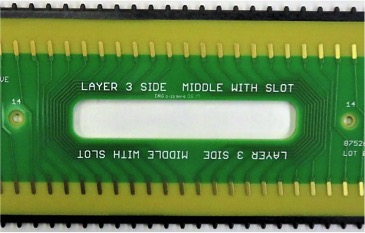
\includegraphics[height=0.28\textheight]{apa-side-board-slot.jpg}
}\quad
\fbox{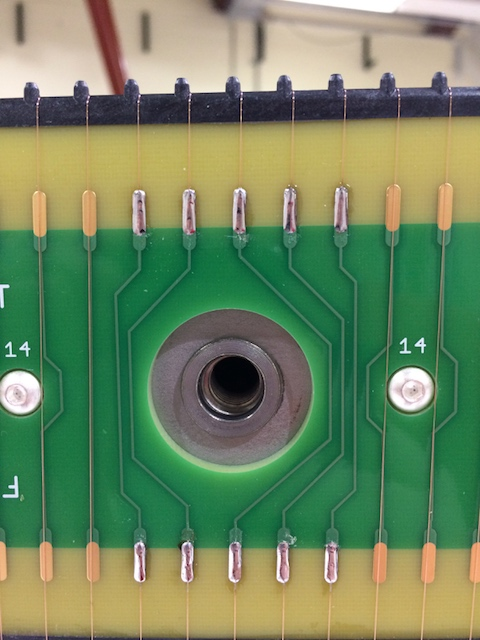
\includegraphics[height=0.28\textheight,trim=0mm 0mm 0mm 25mm,clip]{apa-side-board-round-hole.jpg}
}
\end{dunefigure}

A number of hole or slot features are needed in the edge boards to provide access to the underlying frame (see Figure~\ref{fig:tpc_apa_sideboardmodel} for examples).  In order that these openings not be covered by wires, the sections of wire that would go over the openings are replaced by traces on the boards.  After the wires are wrapped, the wires over the opening are soldered to pads at the ends of the traces and the section of wire between the pads is snipped out.  These traces are easily and economically added to the boards by the many commercial fabricators who make circuit boards. 

The placement of the angled wires are fixed by teeth that are part of an injected molded strip that is glued to the edge of the FR4 boards.  The polymer used for the strips is Vectra e130i (a trade name for 30$\%$ glass filled liquid crystal polymer, or LCP). It retains its strength at cryogenic temperature and has a CTE similar enough to FR4 that differential contraction is not a problem.  The wires make a partial wrap around the pin as they change direction from the face of the \dword{apa} to the edge.

%%%%%%%%%%%%%%%%%%%%%%%%%%%%%%%%%%%%%%%
\subsubsection{Support Combs}
\label{sec:combs}

Support combs are glued at four points along each side of the \dword{apa}, along the four cross beams. These combs maintain the wire and plane spacing along the length of the \dword{apa}. A dedicated jig is used to install the combs and provides the alignment and the pressure to allow the glue to dry. The glue used is the Gray epoxy \num{2216} described below. An eight-hour cure time is required after comb installation on each side of the \dword{apa} before the jig can be removed and production can continue.  Figure~\ref{fig:tpc_apa_sideboardphoto} shows a detail of the wire support combs on a \dword{pdsp} \dword{apa}.

\begin{dunefigure}[Photos of \dword{apa} side boards on the frame]{fig:tpc_apa_sideboardphoto}
{Left: \dword{apa} corner where end boards meet side boards.  The injection molded teeth that guide the $U$ and $V$ wires around the edge are visible at the bottom. Right: The wire support combs.}
\setlength{\fboxsep}{0pt}
\setlength{\fboxrule}{0.5pt}
\fbox{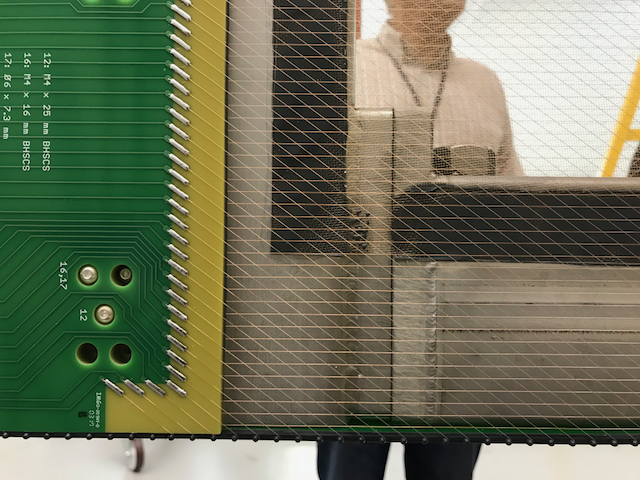
\includegraphics[height=0.3\textheight]{apa-boards-with-pins.png}
}\quad
\fbox{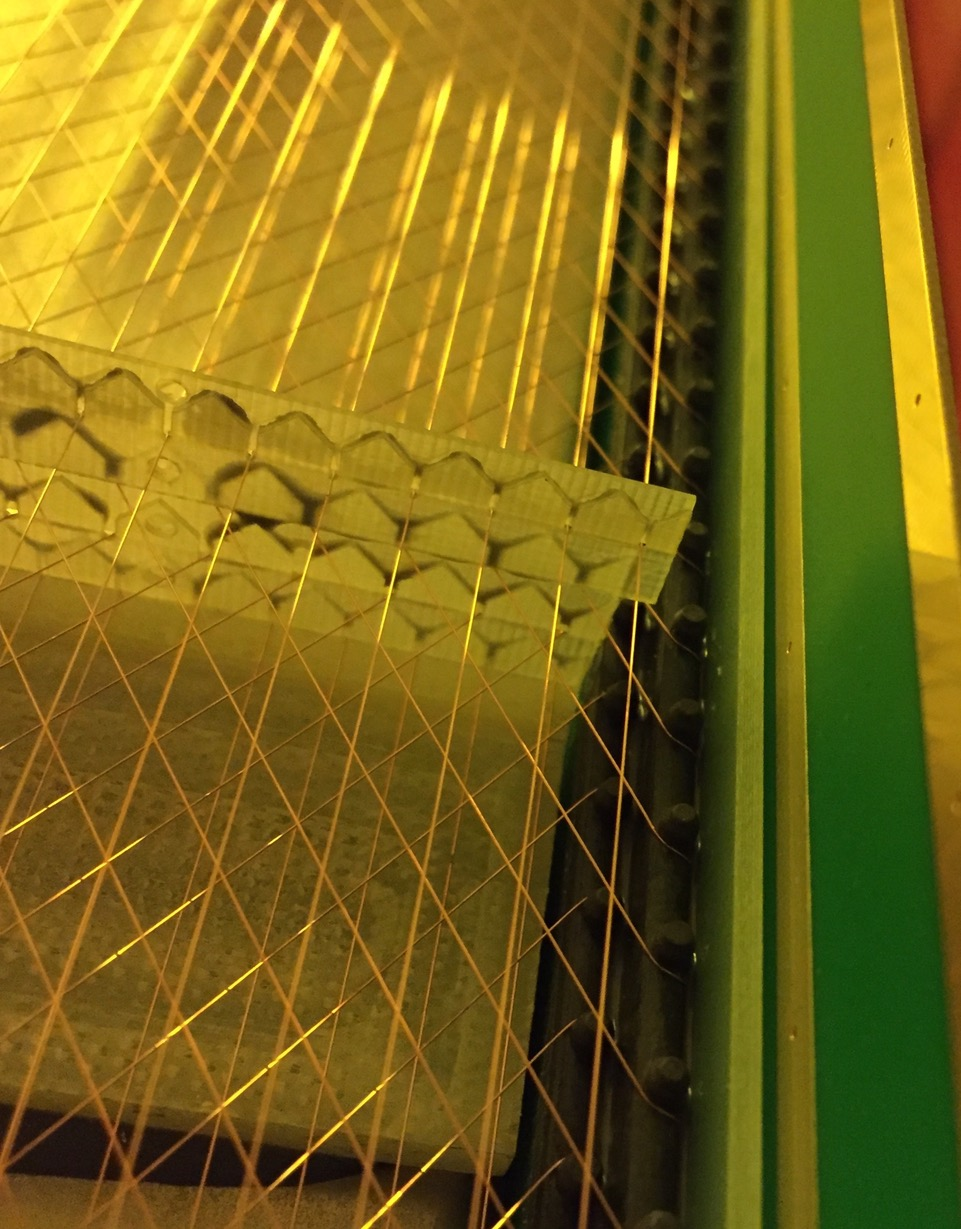
\includegraphics[height=0.3\textheight]{apa-photo-combs.jpg}
}
\end{dunefigure}

%%%%%%%%%%%%%%%%%%%%%%%%%%%%%%%%%%%%%%%
\subsubsection{Solder and Epoxy}
\label{sec:glue-solder}

The ends of the wires are soldered to pads on the edges of the wire boards.  Solder provides both an electrical connection and a physical anchor to the wire pads. A 62$\%$ tin, 36$\%$ lead, and 2$\%$ silver solder was chosen.  A eutectic mix (63/37) is the best of the straight tin-lead 
 solders but the 2$\%$ added silver gives better creep resistance. 

Once a wire layer is complete, the next layer of boards is glued on, this glue providing an additional physical anchor. Gray epoxy \num{2216} by 3M~\footnote{3M\texttrademark \url{https://www.3m.com/}} is used for the glue.  It is strong, widely used (therefore much data is available), and it retains good properties at cryogenic temperatures.  

